\documentclass[a4paper,12pt,oneside,openright,final]{memoir}
\usepackage[table]{xcolor}
\usepackage{graphicx}
\usepackage[latin1]{inputenc}
\usepackage[ruled,vlined]{algorithm2e}
\usepackage{setspace}
\usepackage{url}
\usepackage{amsmath}
\usepackage{mathrsfs}
\usepackage{mathptmx}
\usepackage{amssymb}
\usepackage{bbm}
\usepackage{verbatim}
\usepackage{calc}
\usepackage{multirow}
\usepackage{pagina}
\usepackage{nomes}
\usepackage{pbox}
\usepackage{subcaption}
\usepackage{epstopdf}
\usepackage{subfig}
\usepackage[portuguese]{babel}
\usepackage[
    a4paper,
    portuguese,
    bookmarks=true,
    bookmarksnumbered=true,
    linktocpage,
    ]{hyperref}
\usepackage{memhfixc}
\usepackage{listings}
\usepackage{marvosym}
\usepackage{pgf}
\usepackage{indentfirst}
\usepackage{tikz}
\usetikzlibrary{arrows,automata,positioning,trees,shapes}
\usepackage{mdframed}
\usepackage[T1]{fontenc}
\usepackage{tabu}

\setlrmarginsandblock{3cm}{2cm}{*}
\setulmarginsandblock{3cm}{3cm}{*}
\setheaderspaces{2cm}{*}{*}

\checkandfixthelayout

\makeheadrule{myheadings}{\textwidth}{\normalrulethickness}
\makeoddhead{myheadings}{\textsc{\leftmark}}{}{\thepage}	%

\copypagestyle{contents}{myheadings}
\makeoddhead{contents}{\textsc{\contentsname}}{}{\thepage}

\copypagestyle{bibliography}{myheadings}
\makeoddhead{bibliography}{\textsc{\bibname}}{}{\thepage}

\makeatletter

\def\mychaptermark#1{%
	\markboth{%
	\ifnum \c@secnumdepth >\m@ne
		\if@mainmatter
			\thechapter. \ %
		\fi
	\fi
	#1}{}}%

\def\mysectionmark#1{%
\markright{%
	\ifnum \c@secnumdepth > \z@
		\thesection. \ %
	\fi
	#1}}%

\makeatother

\maxsecnumdepth{subsubsection}

\newcommand{\tableformat}{\small\centering}
\newcommand{\figureformat}{\centering}

\renewcommand{\labelenumi}{\alph{enumi})}
\renewcommand{\labelenumii}{\arabic{enumii}.}

\setcounter{tocdepth}{2} %-- ajusta produndidade do indice

\let\Chapter\chapter
\def\chapter{\addtocontents{lol}{\protect\addvspace{10pt}}\Chapter}

\renewcommand{\lstlistingname}{Algoritmo}
\renewcommand{\lstlistlistingname}{Lista de Algoritmos}

\lstset{
  numbers=left,
  stepnumber=1,
  firstnumber=1,
  numberstyle=\tiny,
  extendedchars=true,
  breaklines=true,
  frame=tb,
  basicstyle=\footnotesize,
  stringstyle=\ttfamily,
  showstringspaces=false,
  captionpos=b,
  breakautoindent=truem
  language=C,
  numbersep=5pt,
  tabsize=2,
  morekeywords={assert,enquanto,se,fim,entao,senao,retorne,faca,assume,Passo,for,int,long, unsigned,while}
}

\makeatletter
\renewcommand\l@lstlisting[2]{\@dottedtocline{1}{0cm}{0.95cm}{#1}{#2}}
\makeatother

\newcolumntype{P}[1]{>{\centering\arraybackslash}p{#1}}

\usepackage{parskip}
\setlength{\parindent}{35pt}


\hyphenation{matema-ticamente moni-torar operacio-nal ESBMC bi-bli-o-te-ca de-ter-mi-n�s-ti-cos mul-ti-pa-ra-dig-mas}

\begin{document}

\newtheorem{definition}{Defini��o}[chapter]
\newtheorem{lemma}{Lemma}[chapter]

\newtheorem{fact}{Fact}[chapter]

\newtheorem{example}{Example}[chapter]

% -- Titulo e Descricao ------------------------------------------------------
\newcommand{\tittese}{%
	\textsf{\bfseries\Large Verifica��o de programas C++ baseados no \textit{framework} cross-plataforma Qt\\
	\vspace{0.8ex}
        }}

\newcommand{\descrtese}{%
\hspace{\stretch{1}}\parbox{0.51\textwidth}{%
Disserta��o apresentada ao Programa de P\'os-Gradua\c{c}\~ao em Engenharia El�trica, como requisito parcial
para obten\c{c}\~ao do T\'{\i}tulo de Mestre em Engenharia El�trica. \'Area de concentra\c{c}\~ao: Automa��o e Controle.
}}

% -- Capa ---------------------------------------------------------------------

\frontmatter
%\doublespacing
%\singlespacing
\pagestyle{empty}

%{centering
\begin{center}

\includegraphics[bb=0 0 646 638,height=2.5cm]{figuras/ufam.png}

\textsf{\large%
Universidade Federal do Amazonas\\
Faculdade de Tecnologia\\
Programa de P\'os-Gradua\c{c}\~ao em Engenharia El�trica}

\vspace*{4cm}
\vspace*{\stretch{1}}

\tittese

\vspace*{4cm}
\vspace*{\stretch{1}}

{\large M�rio Angel Praia Garcia}

\vspace*{3cm}
\vspace*{\stretch{1}}

Manaus -- Amazonas

Abril de 2016
\end{center}

%}
%\cleardoublepage


% -- Contracapa ---------------------------------------------------------------

%{\singlespacing\centering
\begin{center}
{\large M�rio Angel Praia Garcia}

\vspace*{4cm}
\vspace*{\stretch{2}}

\tittese

\vspace*{2cm}
\vspace*{\stretch{1}}

\descrtese

\vspace*{2cm}
\vspace*{\stretch{1}}

Orientador: Lucas Carvalho Cordeiro \\
Coorientador: Waldir Sabino da Silva J�nior
\end{center}

%}
%\cleardoublepage


% -- Banca Examinadora --------------------------------------------------------

%{\singlespacing\centering

\begin{center}
{\large M�rio Angel Praia Garcia}

\vspace*{3cm}
%\vspace*{\stretch{2}}

\tittese

\vspace*{1cm}
%\vspace*{\stretch{1}}

%\descrtese

\vspace*{1cm}
%\vspace*{\stretch{1}}

Banca Examinadora
\vspace{2em}

Prof. Ph.D. Lucas Carvalho Cordeiro -- Orientador\\
Departamento de Eletr�nica e Computa��o -- UFAM
\vspace{2em}

Prof. D.Sc. Waldir Sabino da Silva J�nior -- Presidente e Coorientador\\
Departamento de Eletr�nica e Computa��o -- UFAM
\vspace{2em}

Prof. D.Sc. Raimundo da Silva Barreto \\
Instituto de Computa��o -- UFAM
\vspace{2em}

Prof. D.Sc. Tayana Uch�a Conte \\
Instituto de Computa��o -- UFAM
\vspace{2em}

%\vspace*{1cm}
\vspace*{\stretch{0.5}}

Manaus -- Amazonas

Agosto de 2016

\end{center}
%}
\cleardoublepage

%\cleardoublepage

% -- Dedicat�ria --------------------------------------------------------------

\vspace*{\stretch{2}}

\begin{flushright}
\textit{� minha m�e, av� e tias.}\hspace{1cm}
\end{flushright}

\vspace*{\stretch{1}}

\cleardoublepage

% -- Agradecimentos -----------------------------------------------------------

\chapter*{Agradecimentos}
\thispagestyle{empty}

%{\doublespacing

%\setlength{\parindent}{0cm}

Agrade�o primeiramente a Deus por ter iluminado meu caminho, minhas decis�es e me proporcionado est� oportunidade.

Agrade�o � minha m�e, F�tima Tereza Praia Garcia, por estar sempre do meu lado e cujo amor � incondicional. As minhas tias, Letice e Lenice Praia, por me ajudarem em meu crescimento pessoal e incentivo a n�o desistir dessa jornada e � minha av�, Maria Tereza Praia Soares Lima, por sua paci�ncia, compreens�o, ajuda e pelo seu amor.

Agrade�o aos meus amigos e colegas de mestrado da UFAM, que me ajudaram diretamente e inderetamente nessa jornada, pelo incentivo e apoio dado.

Agrade�o aos amigos e ex-colegas de gradua��o da UEA, pela amizade e companheirismo.

Agrade�o ao Prof. Lucas Cordeiro, pela dedica��o, paci�ncia, encorajamento e apoio oferecido para
a realiza��o desse trabalho.

Agrade�o � equipe do projeto de verifica��o formal na UFAM, que contribu�ram direta e indiretamente para a realiza��o deste trabalho.

\vspace*{3cm}
\cleardoublepage

% -- Ep�grafe -----------------------------------------------------------------

%{\singlespacing
\vspace*{1cm}
\vspace*{\stretch{1}}

\hspace{\stretch{1}}\parbox{0.5\textwidth}{
\begin{flushright}
\emph{``Viver n�o � necess�rio. Necess�rio � criar.''.}
\end{flushright}
}
\vspace{2em}

\hspace{\stretch{1}}{\emph{Fernando Pessoa (1888-1935)}}

\vspace*{\stretch{1}}

%}
%\cleardoublepage

%% -- Resumo -------------------------------------------------------------------
\chapter*{Resumo}
\thispagestyle{empty}

%{\onehalfspacing

O processo de desenvolvimento de software para sistemas embarcados tem crescido rapidamente, o que na maioria das vezes acarreta em um aumento da complexidade associada a esse tipo de projeto. Como consequ�ncia, as empresas de eletr�nica de consumo costumam investir recursos em mecanismos de verifica��o r�pida e autom�tica, com o intuito de desenvolver sistemas robustos e assim reduzir as taxas de \textit{recall} de produtos. Al�m disso, a redu��o no tempo de desenvolvimento e na robustez dos sistemas desenvolvidos podem ser alcan�ados atrav�s de \textit{frameworks} multi-plataformas, tais como Qt, que oferece um conjunto de bibliotecas (gr�ficas) confi�veis para v�rios dispositivos embarcados. Desta forma, este trabalho prop�e uma vers�o simplificada do \textit{framework} Qt, integrado a um verificador baseado nas teorias do m�dulo da satisfatibilidade, denominado \textit{Efficient SMT-Based Bounded Model Checker} (ESBMC++), o qual verifica aplica��es reais que ultilizam o Qt, apresentando uma taxa de sucesso de $89$\%, para os \textit{benchmarks} desenvolvidos. Com a vers�o simplificada do \textit{framework} Qt proposto, tamb�m foi feita uma avalia��o ultilizando outros verificadores que se encontram no estado da arte para verifica��o de programas em C++. Dessa maneira, a metodologia proposta se afirma como a primeira a verificar formalmente aplica��es baseadas no \textit{framework} Qt, al�m de possuir um potencial para desenvolver novas frentes para a verifica��o de c�digo port�til.


\vspace*{\stretch{1}} %texto se adapta para ocupar toda a p�gina

\noindent \textsf{Palavras-chave:} Modelo Operacional, \textit{Framework} Qt, Verifica��o Formal, \textit{Bounded Model Checking}.
%}

\cleardoublepage

%% -- Resumo -------------------------------------------------------------------
\chapter*{Abstract}
\thispagestyle{empty}

%{\onehalfspacing

The software development for embedded systems is getting faster and faster, which generally incurs an increase in the associated complexity. As a consequence, consumer electronics companies usually invest a lot of resources in fast and automatic verification mechanisms, in order to create robust systems and reduce product recall rates. In addition, further development-time reduction and system robustness can be achieved through cross-platform frameworks, such as Qt, which favor the reliable port of software stacks to different devices. Based on that, the present work proposes a simplified version of the Qt framework, which is integrated into a checker based on satisfiability modulo theories (SMT), name as the efficient SMT-based bounded model checker (ESBMC++), for verifying actual Qt-based applications, and presents a success rate of 89\%, for the developed benchmark suite. We also evaluate our simplified version of the Qt framework using other state-of-the-art verifiers for C++ programs and an evaluation about their level of compliance. It is worth mentioning that the proposed methodology is the first one to formally verify Qt-based applications, which has the potential to devise new directions for software verification of portable code.

\vspace*{\stretch{1}} %texto se adapta para ocupar toda a pagina

\noindent \textsf{Keywords:} Operational Model, Qt Framework, Bounded Model Checking, Formal Verification.

%}

\cleardoublepage


% -- �ndices ------------------------------------------------------------------

\pagestyle{contents}
%\pagenumbering{roman}

%\tableofcontents*  % gera o �ndice (sum�rio)
%\cleardoublepage

%\phantomsection
%\addcontentsline{toc}{chapter}{\listfigurename}
%\listoffigures*    % gera a lista de figuras
%\cleardoublepage

%\phantomsection
%\addcontentsline{toc}{chapter}{\listtablename}
%\listoftables*     % gera a lista de tabelas
%\cleardoublepage

%\lstlistoflistings     % gera a lista de tabelas
%\cleardoublepage

%\chapter{Abrevia��es}
\label{appendix:abreviacao}

\noindent \textbf{QtOM}	-	\textit{\textbf{M}odel \textbf{O}perational \textbf{Q}t}  \\
\textbf{IU}	-	\textbf{I}nterface para \textbf{U}su�rio \\
\textbf{MO}	-	\textbf{M}odelo \textbf{O}peracional \\
\textbf{BMC}	-	\textit{\textbf{B}ounded \textbf{M}odel \textbf{C}hecking} \\
\textbf{SMT}	-	\textit{\textbf{S}atisfiability \textbf{M}odulo \textbf{T}heories} \\
\textbf{ESBMC}	-	\textit{\textbf{E}fficient \textbf{S}MT-Based Context-\textbf{B}ounded \textbf{M}odel \textbf{C}hecker} \\
\textbf{VC}	-	\textit{\textbf{V}erification \textbf{C}condition} \\
\textbf{GPU}	-	\textit{\textbf{G}raphics \textbf{P}rocessing \textbf{U}nit} \\
\textbf{SAT}	-	\textit{\textbf{B}oolean \textbf{S}atisfiability} \\
\textbf{LLBMC}	-	\textit{\textbf{L}ow \textbf{L}evel \textbf{B}ounded \textbf{M}odel \textbf{C}hecker} \\
\textbf{STL}	-	\textit{\textbf{S}tandard \textbf{T}emplate \textbf{L}ibrary} \\
\textbf{CBMC}	-	\textit{\textbf{C} \textbf{B}ounded \textbf{M}odel \textbf{C}hecker} \\
\textbf{GCC}	-	\textit{\textbf{GNU} \textbf{C}ompiler \textbf{C}ollection} \\
\textbf{AST}	-	\textit{\textbf{A}bstract \textbf{S}yntax \textbf{T}ree} \\
\textbf{VCG}	-	\textit{\textbf{V}erification \textbf{C}condition \textbf{G}enerator} \\
\textbf{TMS}	-	\textit{\textbf{T}iled \textbf{M}ap \textbf{S}ervice} \\
\textbf{IREP}	-	\textit{\textbf{I}ntermediate \textbf{REP}resentation} \\
\textbf{SSA}	-	\textit{\textbf{S}ingle \textbf{S}tatic \textbf{A}ssignment} \\
\textbf{GUI}	-	\textit{\textbf{G}raphical \textbf{U}ser \textbf{I}nterface} \\
\textbf{LIFO}	-	\textit{\textbf{L}ast-in \textbf{F}irst-out} \\
\textbf{FIFO}	-	\textit{\textbf{F}irst-in \textbf{F}irst-out} \\


\mainmatter
\pagestyle{myheadings}

\let\chaptermark=\mychaptermark
\let\sectionmark=\mysectionmark

%\singlespacing

\setcounter{secnumdepth}{2} %-- ajusta profundidade da contagem de s�ries

%%%%%%%%%%%%%%%%%%%%%%%%%%%%%%%%%%%%%%%%%%%%%%
\chapter{Introdu��o}
\label{chapter:introducao}
%%%%%%%%%%%%%%%%%%%%%%%%%%%%%%%%%%%%%%%%%%%%%%

A atual dissemina��o com rela��o aos sistemas embarcados e sua devida import�ncia est� de acordo com a evolu��o dos componentes de hardware e softwares associados a eles. Na realidade, esses sistemas t�m crescido em rela��o a sua robustez e complexidade, onde se torna vis�vel o uso de processadores com v�rios n�cleos, mem�rias compartilhadas escal�veis entre outros avan�ados recursos, de maneira a suprir o crescimento do poder computacional exigido, no qual pode-se obter por meio da combina��o de linguagens de programa��o e \textit{frameworks}. Neste contexto, o Qt apresenta-se como um poderoso \textit{framework} multi-plataforma para dispostivos, o qual enfatiza a cria��o de interface para usu�rio (IU) e o desenvolvimento de aplica��es gr�ficas~\cite{Qt15}. No entanto, como a complexidade de tais sistemas tende a crescer, o seu (bom) funcionamento se torna dependente do usu�rio; depend�ncia est� que tamb�m cresce de forma r�pida. Em consequ�ncia, a confiabiliadade destes sistesmas torna-se algo de grande import�ncia no processo de desenvolvimento de dispositivos comerciais e suas aplica��es espec�ficas.

Empresas de eletr�nica de consumo cada vez mais investem em tempo e esfor�o para desenvolver alternativas r�pidas e baratas referentes � verifica��o, com o objetivo de verificar a corretude de seus sistemas com o intuito de evitar perdas fincanceiras~\cite{Berard10}. Entre as alternativas j� existentes, uma das mais eficiente e menos custosa � a abordagem da verifica��o de modelos~\cite{Clarke99}~\cite{Christel08}. Por�m, existem muitos sistemas que n�o s�o poss�veis de verific�-los de uma maneira autom�tica devido � falta de suporte de certos tipos de linguagens e \textit{frameworks} por parte dos verificadores de c�digo. Por exemplo, o verificador Java PathFinder � capaz de verificar c�digos em Java baseado em byte-code~\cite{NASA07}, mas n�o h� suporte a verifica��o (completa) de aplica��es Java que utilizam o sistema operacional Android~\cite{MerweMV14}. Na realidade, esta verifica��o somente se torna poss�vel se existir uma representa��o abstrata das bibliotecas associadas, denominada de modelo operacional(MO), que de forma conservadora aproxima-se a sem�ntica usada pelo sistema a ser verificado~\cite{MerweTMV15}.

Este trabalho identifica as principais caracter�sticas do \textit{framework} Qt e prop�e um modelo operacional (MO) que tem como prop�sito analisar e verificar as propriedades relacionadas de acordo com as suas funcionalidades. Os algoritmos desenvolvidos neste trabalho foram intregrados em uma ferramenta de verifica��o de modelos limitada (do ingl�s, \textit{Bounded Model Checking} - BMC) baseada nas teorias do m�dulo da satisfatibilidade (do ingl�s, satisfiability modulo theories - SMT), denominada \textit{Efficient SMT-based Context-Bounded Model Checker} (ESBMC$++$)~\cite{ECBS13}~\cite{ICSE11}~\cite{TSE12}, a fim de verificar as espec�ficas propriedades de programas em Qt/C++. A combina��o entre ESBMC e MOs foi aplicada anteriormente para que se houvesse suporte a programas em C++, conforme descrito por Ramalho \textit{et al}.~\cite{ECBS13}. No entanto, na metodologia proposta, um MO � utilizado para identificar elementos do \textit{framework} Qt e verificar propriedades espec�ficas relacionadas a essas estruturas por meio de pr� e p�s-condi��es~\cite{monteiro2015}.


%%%%%%%%%%%%%%%%%%%%%%%%%%%%%%%%%%%%%%%%%%%%%%
\section{Descri��o do Problema}
%%%%%%%%%%%%%%%%%%%%%%%%%%%%%%%%%%%%%%%%%%%%%%

Descri��o

%%%%%%%%%%%%%%%%%%%%%%%%%%%%%%%%%%%%%%%%%%%%%%
\section{Objetivos}
%%%%%%%%%%%%%%%%%%%%%%%%%%%%%%%%%%%%%%%%%%%%%%

O objetivo geral deste trabalhar � aplicar as t�cnicas de verifica��o utilizando modelos operacionais para checar aplica��es que utilizam o \textit{framework} Qt, usando ferramentas de verifica��o, a fim de validar a cobertura e o comportamento do modelo operacional proposto em rela��o ao \textit{framework} utilizado.

Os objetivos espec�ficos s�o listados a seguir:

\begin{itemize}
  \item Desenvolver uma implementa��o simplificada que oferece estritamente o mesmo comportamento do \textit{framework} Qt com foco na verifica��o de suas propriedades.
  \item Verificar o acesso de mem�ria inv�lida, valores que especificam o tempo, acesso � arquivos ausentes, ponteiros nulos, manipula��o de cadeia de caracteres (\textit{strings}), uso de \textit{containers}, entre outras propriedades de interesse para aplica��es Qt.
  \item Aplicar a metodologia de verifica��o proposta em aplica��es reais que utilizam o \textit{framework} Qt.
\end{itemize}

%%%%%%%%%%%%%%%%%%%%%%%%%%%%%%%%%%%%%%%%%%%%%%
\section{Trabalhos relacionados}
%%%%%%%%%%%%%%%%%%%%%%%%%%%%%%%%%%%%%%%%%%%%%%

De acordo com a atual literatura sobre verifica��o, n�o existe outro verificador dispon�vel que seja capaz de verificar funcionalidades do \textit{framework} Qt. Ao contr�rio, as aplica��es de eletr�nica de consumo que utilizam este \textit{framework}, apresentam diversas propriedades que devem ser verificadas como estouro aritm�tico, seguran�a de ponteiros, limite de vetores e corretude no uso de \textit{containers}. Al�m disso, a verifica��o por meio de testes manuais � um processo �rduo e custoso~\cite{monteiro2015}. Em resumo, a t�cnica BMC aplicada em verifica��o de software � usada em diversos verificadores~\cite{FalkeMS13,CBMC14,TSE12,WangBW14} e est� se tornando cada vez mais popular, principalmente, devido ao aumento de solucionadores SMT cada vez mais sofisticados, os quais s�o baseados em eficientes solucionadores de satisfa��o Booleana (do ingl�s, Boolean Satisfiability - SAT)~\cite{Z308}.

Ramalho \textit{et al.}~\cite{ECBS13} apresentam o \textit{Efficient SMT-Based Context-Bounded Model Checker} (ESBMC) como um verificador de modelos limitados para verificar programas em C$++$, sendo denominado ESBMC$++$. ESBMC$++$ utiliza seus modelos operacionais para oferecer suporte � verifica��o das caracter�sticas mais complexas que a linguagem oferece, como \textit{containers} e tratamento de exce��o. Vale ressaltar que os modelos usados s�o uma representa��o abstrata das bibliotecas padr�es do C++, que de forma conservadora se aproximam semanticamente das bibliotecas originais. ESBMC$++$ se utiliza disso para codificar as condi��es de verifica��o criadas usando diferentes teorias de base apoiadas por solucionadores SMT.

Merz, Falke e Sinz~\cite{FalkeMS13} apresentam o \textit{Low-Level Bounded Model Checker} (LLBMC) como um verificador que utiliza modelos operacionais para verificar programas baseados em ANSI-C/C++. LLBMC tamb�m usa um compilador denominado \textit{low level virtual machine} (LLVM) que possui o objetivo de converter programas ANSI-C/C++ em uma representa��o intermedi�ria utilizada pelo verificador. De forma semelhante, ao ESBMC$++$, Merz, Falke e Sinz tamb�m utilizam solucionadores SMT para analisar as condi��es de verifica��o. Contudo, diferente da abordagem aqui proposta, o LLBMC n�o suporta tratamento de exce��o, o que acarreta numa verifica��o incorreta de programas reais escritos em C++, como por exemplo, programas baseados nas bibliotecas de template padr�o (do ingl�s, Standard Template Libraries - STL). Vale ressaltar que a representa��o intermedi�ria usado pelo LLVM perde algumas informa��es sobre a estrutura original dos respectivos programas em C++ , como por exemplo, as rela��es entre classes.

Barnat \textit{et al.} apresenta o DIVINE~\cite{BBH13} como um verificador de modelo de estado expl�cito para programas ANSI-C/C++ sequencias e multi-tarefas, o qual possui como objetivo principal verificar a seguran�a de propriedades de programas ass�ncronos e aqueles que utilizam mem�ria compartilhada. DIVINE faz uso de um compilador conhecido como Clang~\cite{CLANG} como front-end, a fim de converter programas C++ em uma representa��o intermedi�ria utilizada pelo LLVM, que logo em seguida realiza a verifica��o sobre o \textit{byte-code} produzido. Embora o DIVINE possua uma implementa��o de ANSI-C e das bibliotecas padr�es do C++, o que lhe permite verificar programas desenvolvidos com essas linguaguens, o mesmo n�o possui qualquer suporte � representa��o disponibilizada pelo \textit{framework} Qt. De acordo com a abordagem proposta, DIVINE � capaz de criar um programa que possa ser interpretado totalmente pelo LLVM e ent�o ser verificado logo em seguida.

Blanc, Groce e Kroening descrevem a verifica��o de programas em C++ que usam \textit{containers} STL atrav�s de abstra��o de predicados~\cite{Blanc07}, com o uso de tipo de dados abstrato, sendo usados para realizar a verifica��o de STL ao inv�s de usar a implementa��o real dos componentes STL. Na verdade, os autores mostram que a corretude pode ser realizada atrav�s de modelos operacionais, provando que a partir de condi��es pr�vias sobre opera��es, no mesmo modelo, acarreta em condi��es pr�vias nas bibliotecas padr�es, e p�s-condi��es podem ser t�o significativas quanto as condi��es originais. Tal abordagem � eficiente em encontrar erros triviais em programas em C++, mas que necessita de uma pesquisa mais profunda para evitar erros e opera��es enganosas (isto �, ao envolver a modelagem de m�todos internos). Vale ressaltar que, no presente trabalho, simula��es do comportamento de certos m�todos e fun��es superam o problema mencionado (ver Se��o~\ref{sec:preconditions}).

O \textit{C Bounded Model Checker} (CBMC) implementa a t�cnica BMC para programas ANSI-C/C++ por meio de solucionadores SAT/SMT~\cite{CBMC14}. Vale ressaltar que ESBMC foi constru�do a partir do CBMC, portanto, ambos verificadores possuem processos de verifica��o semelhantes. Na verdade, CBMC processa programas C/C++ usando a ferramenta goto-cc~\cite{Wintersteiger09}, a qual compila o c�digo fonte da aplica��o para um \textit{GOTO-programs} equivalente (ou seja, um grafo de fluxo de controle), a partir de um modelo comp�tivel ao GCC. A partir de \textit{GOTO-programs}, o CBMC cria uma �rvore abstrata de sintaxe (do ingl�s, \textit{Abstract Syntax Tree} - AST) que � convertida em um formato independente da linguaguem interna usada para as etapas restantes. O CBMC tamb�m utiliza duas fun��es recursivas ${\cal C}$ e ${\cal P}$ que registram as \emph{restri��es} (ou seja, premissas e atribui��es de vari�veis) e as \emph{propriedades} (ou seja, condi��es de seguran�a e premissas definidas pelo o usu�rio), respectivamente. Este verificador cria de forma autom�tica as condi��es de seguran�a que verificam o estouro aritm�tico, viola��o no limite dos vetores e checagem de ponteiro nulo~\cite{Sites74}. Por fim, um gerador de condi��es de verifica��o (do ingl�s, \textit{Verification Condition Geneator} - VCG) cria condi��es de verifica��o (do ingl�s, Verification Conditions - VCs) a partir das f�rmulas criadas e os envia para um solucionador SAT/SMT. Embora o CBMC esteja relacionado como susposto verificador de programas em C++, Ramalho \textit{et al.}~\cite{ECBS13} e Merz \textit{et al.}~\cite{Florian12} relatam que o CBMC falha ao verificar diversas aplica��es simples em C++, o que tamb�m foi confirmado neste trabalho (ver Se��o~\ref{sec:evaluation}).

Finalmente, destaca-se que o QtOM est� completamente escrito na linguagem de programa��o C++, o que facilita a integra��o dentro de processos de verifica��o de outros verificadores. No presente trabalho, QtOM n�o foi somente intregado ao ESBMC$++$, mas tamb�m no DIVINE~\cite{BBH13} e LLBMC~\cite{FalkeMS13}, afim de obter uma avalia��o mais justa sobre a abordagem proposta.

%%%%%%%%%%%%%%%%%%%%%%%%%%%%%%%%%%%%%%%%%%%%%%
\section{Contribui��es}
%%%%%%%%%%%%%%%%%%%%%%%%%%%%%%%%%%%%%%%%%%%%%%

O trabalho � uma extens�o de trabalhos j� publicados anteriormente~\cite{monteiro2015}. O respectivo modelo operacional(MO) proposto foi ampliado com o objetivo de incluir novas funcionalidades dos principais m�dulos do Qt, neste caso em particular, \textit{QtGui} e \textit{QtCore}. De fato, as principais contribui��es aqui s�o:

\begin{itemize}
  \item Suportar \textit{containers} baseados em templates sequenciais e associativos;
  \item Integrar o modelo operacional proposto denominado QtOM ao processo de verifica��o de programas em C++ em verificadores que se encontram no estado da arte, neste caso, DIVINE~\cite{BBH13} e LLBMC~\cite{FalkeMS13};
  \item Fornecer suporte � verifica��o de duas aplica��es baseadas em Qt denominadas Locomaps~\cite{locomaps} e Geomessage~\cite{geomessage}, respectivamente.
  \item Avaliar o desempenho de tr�s solucionadores SMT(Z3~\cite{Z308}, Yices~\cite{Dutertre:cav2014} e Boolector~\cite{Boolector09}) sobre o conjunto de \textit{benchmarks} utilizados extensivamente e ampliado em rela��o ao trabalho anterior~\cite{monteiro2015} juntamente com a abordagem proposta. 
\end{itemize}

Por fim, em particular, foram inclu�das representa��es para todas as bibliotecas relacionadas com as classes de Qt \textit{containers}. De acordo com o conhecimento atual em verifica��o de software, n�o h� outro verificador que utilize modelos e se aplique t�cnicas BMC para verificar programas baseados no \textit{framework} Qt sobre dispositivos de eletr�nica de consumo.


%%%%%%%%%%%%%%%%%%%%%%%%%%%%%%%%%%%%%%%%%%%%%%
\section{Organiza��o da Disserta��o}
%%%%%%%%%%%%%%%%%%%%%%%%%%%%%%%%%%%%%%%%%%%%%%

Neste cap�tulo, inicialmente descreveram-se sobre o contexto que envolve o trabalho, a motiva��o, seus objetivos e al�m de terem sido apresentados trabalhos relacionados de acordo com a abordagem proposta, com o intuito de descrever refer�ncias sobre o tema proposto. Este trabalho est� organizado da seguinte forma: 

\begin{itemize}
	\item O Cap�tulo 2 apresenta uma breve introdu��o sobre a arquitetura de ESBMC$++$ e as teorias do m�dulo da satisfatibilidade (SMT), al�m de descrever um resumo sobre o \textit{framework} multiplataforma Qt;
	\item O Cap�tulo 3 descreve uma representa��o simplificada das bibliotecas Qt, nomeado como Qt Operational Model (QtOM), que tamb�m aborda pr� e p�s-condi��es.
	\item O Cap�tulo 4 descreve a implementa��o formal de Qt \textit{Containers} associativos e sequencias desenvolvidos de forma detalhada.
	\item O Cap�tulo 5, descreve os resultados experimentais realizados usando benchmarks Qt/C++ e tamb�m a verifica��o de duas aplica��es baseadas em Qt, onde a primeira apresenta imagens de sat�lites, terrenos, mapas de ruas e \textit{Tiled Map Service} (TMS) \textit{panning} entre outras caracter�sticas~\cite{locomaps} e a segunda aplica��o cria um \textit{broadcast User Datagram Protocol} (UDP) baseado em arquivos XML.
	\item Por fim, o Cap�tulo 6 apresenta as conclus�es, destacando a import�ncia da cria��o de um modelo para verificar aplica��es que utilizam framework Qt, assim como, os trabalhos futuros tamb�m s�o descritos.
\end{itemize}
%%%%%%%%%%%%%%%%%%%%%%%%%%%%%%%%%%%%%%%%%%%%%%
\chapter{Fundamenta��o Te�rica}
\label{chapter:background}
%%%%%%%%%%%%%%%%%%%%%%%%%%%%%%%%%%%%%%%%%%%%%%

Este cap�tulo descreve a arquitetura de ESBMC++ e algumas caracter�sticas estruturais do \textit{framework} multiplataforma Qt. Este trabalho consiste na verifica��o de programas em C$++$ baseados no \textit{framework} Qt, usando a ferramenta ESBMC$++$, a qual possui um \textit{front-end} baseado em CBMC com o intuito de produzir VCs para um programa Qt/C$++$. No entanto, em vez de passar tais VCs para um solucionador SAT, o ESBMC$++$ os codifica por meio de diferentes teorias de base do SMT e em seguida, passa os resultados associados para um solucinador SMT.

%%%%%%%%%%%%%%%%%%%%%%%%%%%%%%%%%%%%%%%%%%%%%%
\section{ESBMC++}
\label{sec:arch}
%%%%%%%%%%%%%%%%%%%%%%%%%%%%%%%%%%%%%%%%%%%%%%

O ESBMC$++$ � um \textit{context-bounded model checker} baseado em solucionadores SMT para verificar programas ANSI-C/C$++$~\cite{ECBS13,TSE12,ICSE11,Morse2013}. A Figura~\ref{figure:Fig1} apresenta a arquitetura do ESBMC$++$. Em especial, o ESBMC$++$ verifica programas sequencias e multi-tarefas e analisa propriedades relacionadas � estouro aritm�ticow, divis�o por zero, ind�ces de vetor fora do limite, seguran�a de ponteiros, bloqueio fatal e corrida de dados. No ESBMC$++$, o processo de verifica��o se encontra totalmente autom�tico, isto �, todos os processos realizados s�o representados nas caixas cinzas de acordo com a Figura~\ref{figure:Fig1}, ou seja, n�o existe nenhuma possibilidade do usu�rio pr�-processar programas em qualquer fase descrita~\cite{Morse2014,MorseHandling2013}.

\begin{figure}[htb]
  \centering
  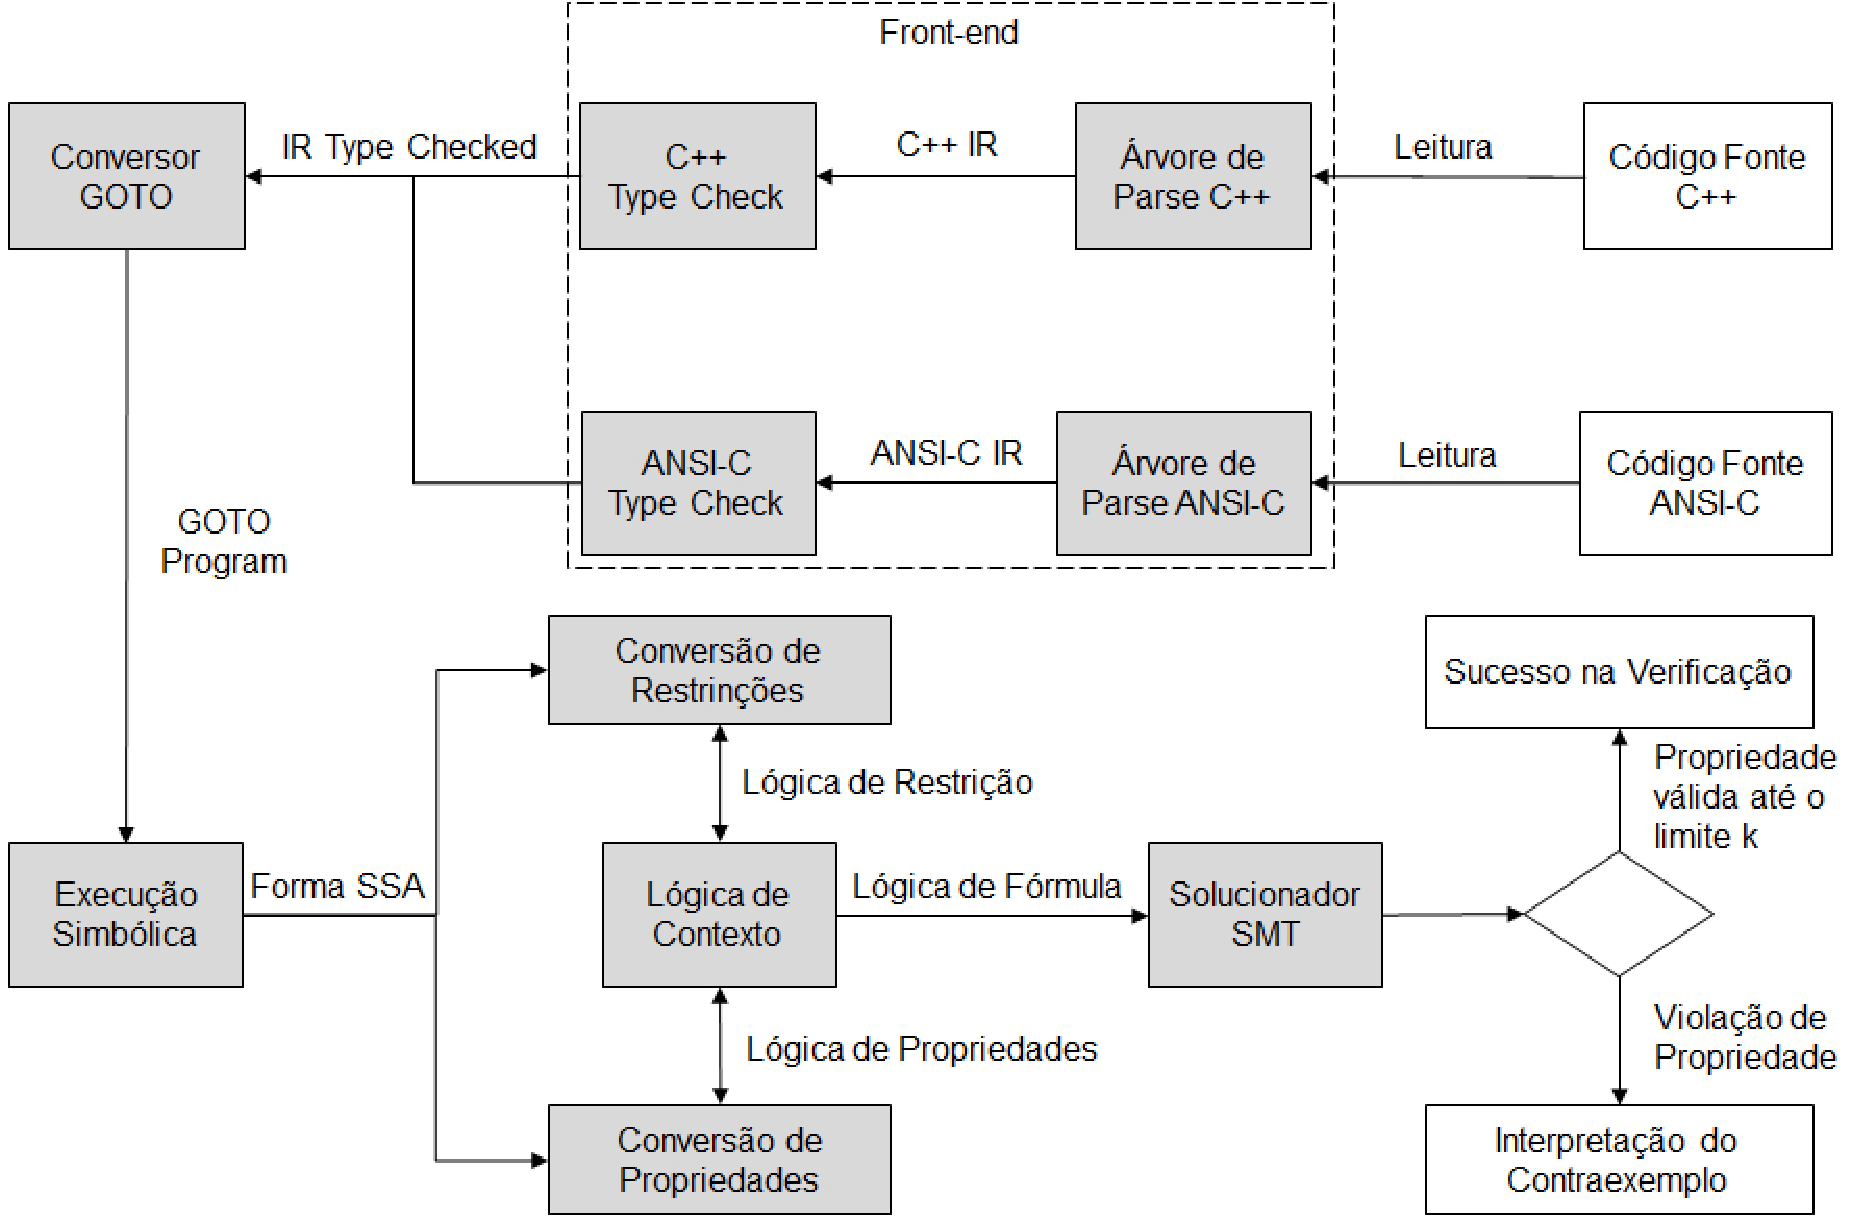
\includegraphics[width=4in]{figuras/Fig1.pdf}
  \caption{Vis�o geral da arquitetura do ESBMC$++$.}
  \label{figure:Fig1}
\end{figure}

Durante o processo de verifica��o, primeiramente � realizado o \textit{parser} do c�digo fonte a ser analisado. Na verdade, o \textit{parser} utilizado no ESBMC$++$ � fortemente baseado no compilador GNU C$++$~\cite{ECBS13}, uma vez que a abordagem permite que o ESBMC$++$ encontre a maioria dos erros de sintaxe j� relatados pelo GCC. Programas ANSI-C/C$++$/Qt s�o convertidos em uma �rvore de representa��o interm�diaria (do ingl�s, Intermediate Representation - IRep), e boa parte dessa representa��o criada � usada como base para os passos restantes da verifica��o. Vale ressaltar que o modelo operacional (MO) � o ponto chave neste processo de convers�o, o que ser� explicado no Cap�tulo~\ref{chapter:smt-bmc}.

Na etapa seguinte, denominada \textit{type-checking}, verifica��es adicionais s�o realizadas, na �rvore IRep, que incluem atribui��es, \textit{type-cast}, inicializa��o de ponteiros e a an�lise das chamadas de fun��o, assim como, a cria��o de templates e instancia��es~\cite{ECBS13}. Em seguida, a �rvore IRep � convertida em express�es \textit{goto} que simplificam a representa��o das instru��es (por exemplo, a substitui��o de \textit{while} por \textit{if} e instru��es \textit{goto}) e s�o executadas de forma simb�lica por \textit{GOTO-symex}). Como resultado, uma atribui��o est�tica �nica (do ingl�s, Single Static Assignment - SSA) � criada. Baseado nisso, o ESBMC++ cria duas f�rmulas chamadas \textit{restri��es} (ou seja, premissas e atribui��es de vari�veis) e \textit{propriedades} (ou seja, condi��es de seguran�a e premissas definidas pelo o usu�rio) consideradas fun��es recursivas. Essas f�rmulas acumulam predicados de fluxo de controle de cada ponto do programa analisado e os usa para armazernar restri��es (f�rmula ${\cal C}$) e propriedades (f�rmula ${\cal P}$), de modo que reflita adequadamente a sem�ntica do programa. Posteriormente, essas duas f�rmulas de l�gica de primeira ordem s�o verificadas por um solucinador SMT.

Por fim, se uma viola��o em alguma propriedade for encontrada, um contraexemplo � gerado pelo ESBMC++~\cite{Cordeiro2012}, o qual atribui valores as vari�veis de programa com o intuito de reproduzir o erro encontrado. De fato, contraexemplos possuem grande import�ncia para o diagn�stico e a an�lise da execu��o do programa, dado que as viola��es encontradas pode ser sistematicamente rastreadas~\cite{RochaBCN12}.

%%%%%%%%%%%%%%%%%%%%%%%%%%%%%%%%%%%%%%%%%%%%%%
\section{Satisfiability Modulo Theories (SMT)}
%\section{Teorias do M�dulo da Satisfabilidade}
%%%%%%%%%%%%%%%%%%%%%%%%%%%%%%%%%%%%%%%%%%%%%%

SMT determina a satisfatibilidade das f�rmulas expressas em l�gica de primeira ordem, usando uma combina��o de suas teorias, a fim de generalizar a satisfabilidade proposicional, dando suporte � fun��es n�o interpretadas, aritm�tica linear e n�o linear, vetores de bit, tuplas, vetores e outras teorias de primeira ordem. Dado uma teoria ${\cal T}$ e uma f�rmula livre de quantificadores $\psi$, a respectiva f�rmula, � satisfat�vel ${\cal T}$ se somente se existir uma estrutura que satisfa�a tanto a f�rmula quanto as senten�as de ${\cal T}$, ou seja, se ${\cal T}\cup \{\psi\}$ � satisfat�vel~\cite{Bradley07}. Dado um conjunto $\Gamma\cup \{\psi\}$ das f�rmulas sobre ${\cal T}$, $\psi$ � uma consequ�ncia ${\cal T}$ de $\Gamma$ ($\Gamma\models_{\cal T}\psi$) se e somente se todo os modelos de ${\cal T}\cup\Gamma$ � tamb�m um modelo de $\psi$. Desta forma, ao verificar $\Gamma\models_{\cal T}\psi$ pode se reduzi-la para verifica��o de um satisfat�vel $\cal T$ de $\Gamma\cup\{\neg\psi\}$.

As teorias dos vetores dos solucinadores SMT s�o normalmente baseadas em axiomas de McCarthy~\cite{McCarthy62}. A fun��o \emph{select(a,i)} indica o valor de $a$ no �ndice $i$ e a fun��o \emph{store(a,i,v)} indica um vetor que � exatamente o mesmo que $a$, a menos que o valor do �ndice $i$ seja $v$. Formalmente,\emph{select} e \emph{store} pode ent�o ser caracterizados por axiomas~\cite{Z308,Boolector09,CVC07}

\[
\begin{array}{l}
 i=j  \Rightarrow select\left(store\left(a,i,v\right),j\right)=v \\
\end{array}
\]

{\noindent e}

\[
\begin{array}{l}
 i \neq j \Rightarrow select\left(store\left(a,i,v\right)=select\left(a,j\right).
\end{array}
\]

\noindent
Tuplas s�o utilizadas para modelar \textit{union} e \textit{struct} em ANSI-C, al�m de fornecer as opera��es de \textit{store} e \textit{select}, as quais s�o semelhantes as usadas em vetores. No entanto, elas trabalham com elementos de tupla, isto �, cada campo de uma tupla � representado por uma constante inteira. Desta forma, a express�o $\mathit{select}(t, f)$ indica o campo $f$ de uma tupla $t$, enquanto a express�o $\mathit{store}(t, f, v)$ indica uma tupla $t$ que, no campo $f$, tem o valor $v$. A fim de analisar a satisfabilidade de uma determinada f�rmula, solucianadores SMT lidam com termos baseados em suas teorias usando um procedimento de decis�o~\cite{MouraB09}.

%=-=-=-=-=-=-=-=-=-=-=-=-=-=-=-=-=-=-=-=-=-=-=-=-=-=-=
\section{O Framework Multiplataforma Qt}
%=-=-=-=-=-=-=-=-=-=-=-=-=-=-=-=-=-=-=-=-=-=-=-=-=-=-=

Diversos m�dulos de software, conhecidos como \textit{frameworks}, t�m sido utilizados para acelerar o processo de desenvolvimento de aplica��es. Diante desse contexto, o \textit{framework} multiplataforma Qt~\cite{Qt15} representa um bom exemplo de um conjunto de classes reutilizav�is, onde a engenharia de software presente � capaz de favorecer o desenvolvimento de aplica��es gr�ficas que utilizam C++~\cite{Qt15} e Java~\cite{qtjambi}. S�o fornecidos programas que s�o executados em diferentes plataformas tanto de hardware quanto de software com o m�nimo de munda�as nas aplica��es desenvolvidas com o objetivo de manter o mesmo desempenho. Samsung~\cite{Samsung}, Philips~\cite{Philips} e Panasonic~\cite{Panasonic} s�o alguma das empresas presentes na lista top $10$ da Fortune $500$ que utilizam Qt para o desenvolvimento de suas aplica��es~\cite{Qt15}.

De acordo com o relat�rio do \textit{Cross-Platform Tool Benchmarking} 2014~\cite{cross2014}, Qt � o \textit{framework} multiplataforma que lidera o desenvolvimento de aplica��es para dispositivos e interfaces para usu�rios. Com as suas bibliotecas organizadas em m�dulos conforme mostrado na Figura~\ref{figure:Fig4}, o m�dulo \textit{QtCore}~\cite{Qt15} � considerado um m�dulo base de Qt, pois, cont�m todas as classes n�o gr�ficas das classes \textit{core} e em particular cont�m um conjunto de bibliotecas denominado de classes \textit{Containers} que possui como implementa��o um modelo base para esses tipos de classe, com um intuito de uso geral ou como uma alternativa para \textit{containers} STL. Esses tipos de estruturas s�o amplamentes conhecidos e usados em aplica��es reais com Qt e consistem em um item muito importante nos processos de verifica��o.

\begin{figure}[htb]
  \centering
  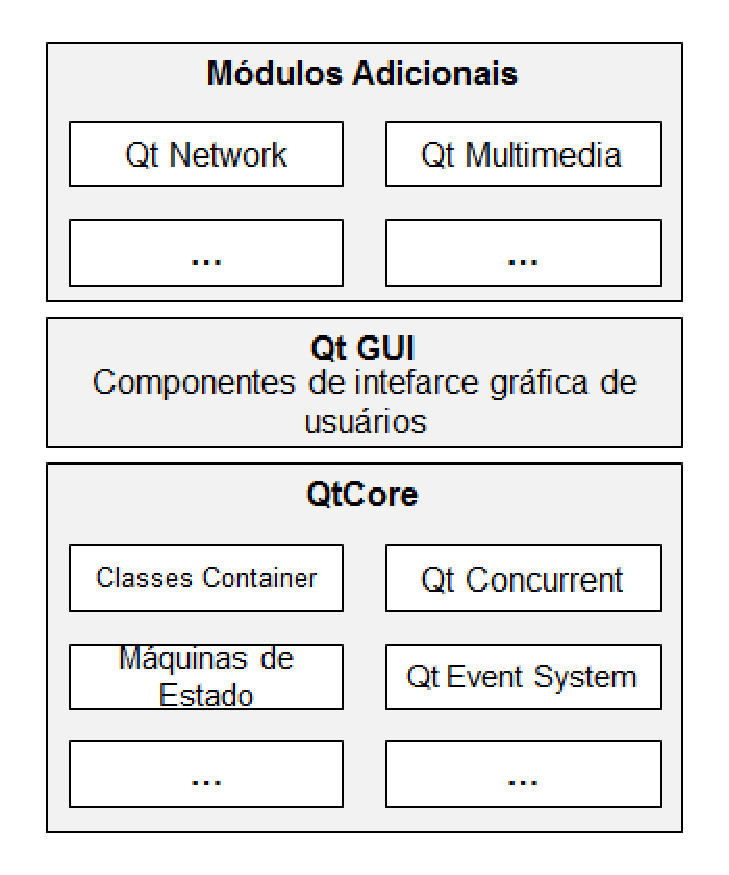
\includegraphics[width=2.0in]{figuras/Fig4.pdf}
  \caption{Vis�o geral da estrutura do \textit{framework} Qt.}
  \label{figure:Fig4}
\end{figure}

Al�m desses subm�dulos, o \textit{QtCore} tamb�m cont�m um sistema de eventos denominado Qt \textit{Event}, onde, Qt representa um evento por meio de um objeto que herda a classe \textit{QEvent} (classe base para o sistema Qt \textit{Event}) na qual cont�m informa��es necess�rias sobre todas as a��es (internas ou externas) relacionadas a uma dada aplica��o. Uma vez instanciado, este objeto � enviado para uma inst�ncia da classe \textit{QObject}, o qual possui como fun��o chamar um m�todo escalonador apropriado para o seu tipo.

Desta forma, o \textit{framework} Qt fornece uma completa abstra��o para aplica��es que envolvem interface gr�fica com o usu�rio (do ingl�s, \textit{Graphical User Interface} - GUI) usando APIs nativas, a partir das diferentes plataformas operacionais disponiv�is no mercado, para consultar as m�tricas e desenhar os elementos gr�ficos. Tamb�m s�o oferecidos \textit{signals} e \textit{slots} com o objetivo de realizar a comunica��o entres os objetos criados~\cite{QtLibs5}. Outra caracter�stica importante a ser ressaltada deste \textit{framework} � a presen�a de um compilador denominado \textit{MetaObject}, o qual � respons�vel por interpretar os programas criados e gerar um c�digo em C++ com meta informa��es~\cite{Moc}.

Por fim e de acordo com o apresentado, nota-se que a complexidade e robustez de programas que utilizam o \textit{framework} Qt afeta diretamente os processos de verifica��o relacionados a eles. Em resumo, o QtOM possui uma representa��o de todas as classes acima referidas e suas respectivas intera��es a fim de suportar tamb�m todo o sistema Qt \textit{Event}.


%%%%%%%%%%%%%%%%%%%%%%%%%%%%%%%%%%%%%%%%%%%%%%
\section{Resumo}
%%%%%%%%%%%%%%%%%%%%%%%%%%%%%%%%%%%%%%%%%%%%%%

Neste cap�tulo, foi descrito a arquitetura de ESBMC$++$ sendo explicado o objetivo e a tarefa de cada etapa de seu processo de verifica��o de acordo como mostrado na figura~\ref{figure:Fig1}, descreveu-se tamb�m como as t�cnicas SMT s�o usadas para determinar a satisfatibilidade das f�rmulas expressas em l�gica de primeira ordem e por fim, foi descrito algumas caracter�sticas estruturais do \textit{framework} multiplataforma Qt.
%%%%%%%%%%%%%%%%%%%%%%%%%%%%%%%%%%%%%%%%%%%%%%
\chapter{M�todo proposto}
\label{chapter:smt-bmc}
%%%%%%%%%%%%%%%%%%%%%%%%%%%%%%%%%%%%%%%%%%%%%%

Este cap�tulo descreve todo o processo de verifica��o de ESBMC$++$ junto com QtOM, cujo torna poss�vel a verifica��o de aplica��es escritas em C$++$ que utilizam o \textit{framework} Qt, e o processo de cria��o de QtOM, enfatizando as classes \textit{containers} do \textit{framework} Qt. Vale ressaltar que ESBMC$++$ apenas suporta a verifica��o de aplica��es ANSI-C/C$++$ que apesar das aplica��es utilizarem C$++$ o \textit{framework} Qt possui suas bibliotecas nativas, as quais possuem estruturas hier�rquicas que inviabilizam a utiliza��o da ferramenta. Inicialmente, na Se��o~\ref{sec:introdutions} � descrito como QtOM auxilia ESBMC$++$ a transformar o c�digo de entrada em uma �rvore IRep e a identificar cada estrutura presente na aplica��o e como est� disposto as classes containers no \textit{framework} Qt, assim como, o seu uso em aplica��es. Logo em seguida, nas Se��es~\ref{sec:preconditions} e~\ref{sec:postconditions} � descrito como QtOM se utiliza de pr� e p�s-condi��es para se obter um comportamento igual ao descrito na documenta��o do \textit{framework} Qt~\cite{Qt15}. Na Se��o~\ref{sec:language} � descrito a linguagem que foi utilizada como base para se criar as representa��es contidas em QtOM com o objetivo de formalizar a implementa��o de cada \textit{container}. Por fim, nas Se��es~\ref{sec:sequential} e~\ref{sec:associative} � descrito como as classes containers foram divididas entre sequenciais e associativas, e o seu comportam no momento de sua utiliza��o por QtOM atrav�s de l�gica formal.


%%%%%%%%%%%%%%%%%%%%%%%%%%%%%%%%%%%%%%%%%%%%%%
\section{Introdu��o}
\label{sec:introdutions}
%%%%%%%%%%%%%%%%%%%%%%%%%%%%%%%%%%%%%%%%%%%%%%
\textcolor{red}{Necess�rio reler e reescrever essa se��o}

Inicialmente, o \textit{parser} utilizado j� havia sido mencionado na Se��o~\ref{sec:arch} do Cap�tulo~\ref{chapter:background} e, nesta etapa, � onde o ESBMC$++$ transforma o c�digo de entrada em uma �rvore IRep, a qual, possui todas as informa��es necess�rias para o processo de verifica��o e, ao fim desta etapa, o ESBMC++ identifica cada estrutura presente no respectivo programa. No entanto, o ESBMC$++$ suporta apenas a verifica��o de programas ANSI-C/C$++$. Apesar dos c�digos analisados do Qt serem escritos em C$++$, suas bibliotecas nativas possuem muitas estruturas hier�rquicas e complexas. Desta maneira, o processo de verifica��o para essas bibliotecas e suas respectivas implementa��es otimizadas afetariam de forma desnecess�ria as VCs, al�m do mais poderiam n�o conter qualquer afirma��o a cerca de propriedades espec�ficas, tornando a verifica��o uma tarefa invi�vel.

O uso do QtOM neste cap�tulo possui como objetivo solucionar o problema descrito acima, por ser uma representa��o simplificada, a qual considera a estrutura de cada biblioteca e suas respectivas classes associadas, incluindo atributos, assinaturas de m�todos, prot�tipos de fun��es e assertivas, garantindo assim que cada propriedade seja formalmente verificada. Na verdade, existem muitas propriedades a serem verificadas como acesso de mem�ria inv�lida, valores negativos que representam per�odos de tempo, acesso � arquivos inexistentes e ponteiros nulos, juntamente com pr� e p�s-condi��es que s�o necess�rias para executar corretamente os m�todos do Qt. Vale ressaltar que QtOM � ligado de forma manual ao ESBMC$++$, logo no in�cio do processo de verifica��o, como mostrado na Figura~\ref{figure:Fig2}. Desta forma, o QtOM pode auxiliar no processo de \textit{parser} durante a cria��o de uma representa��o intermedi�ria em C$++$ que possui todas as assertivas indispens�veis para a verifica��o das propriedades mencionadas acima. Por fim, o fluxo de verifica��o segue de maneira tradicional.

\begin{figure}[htb]
  \centering
  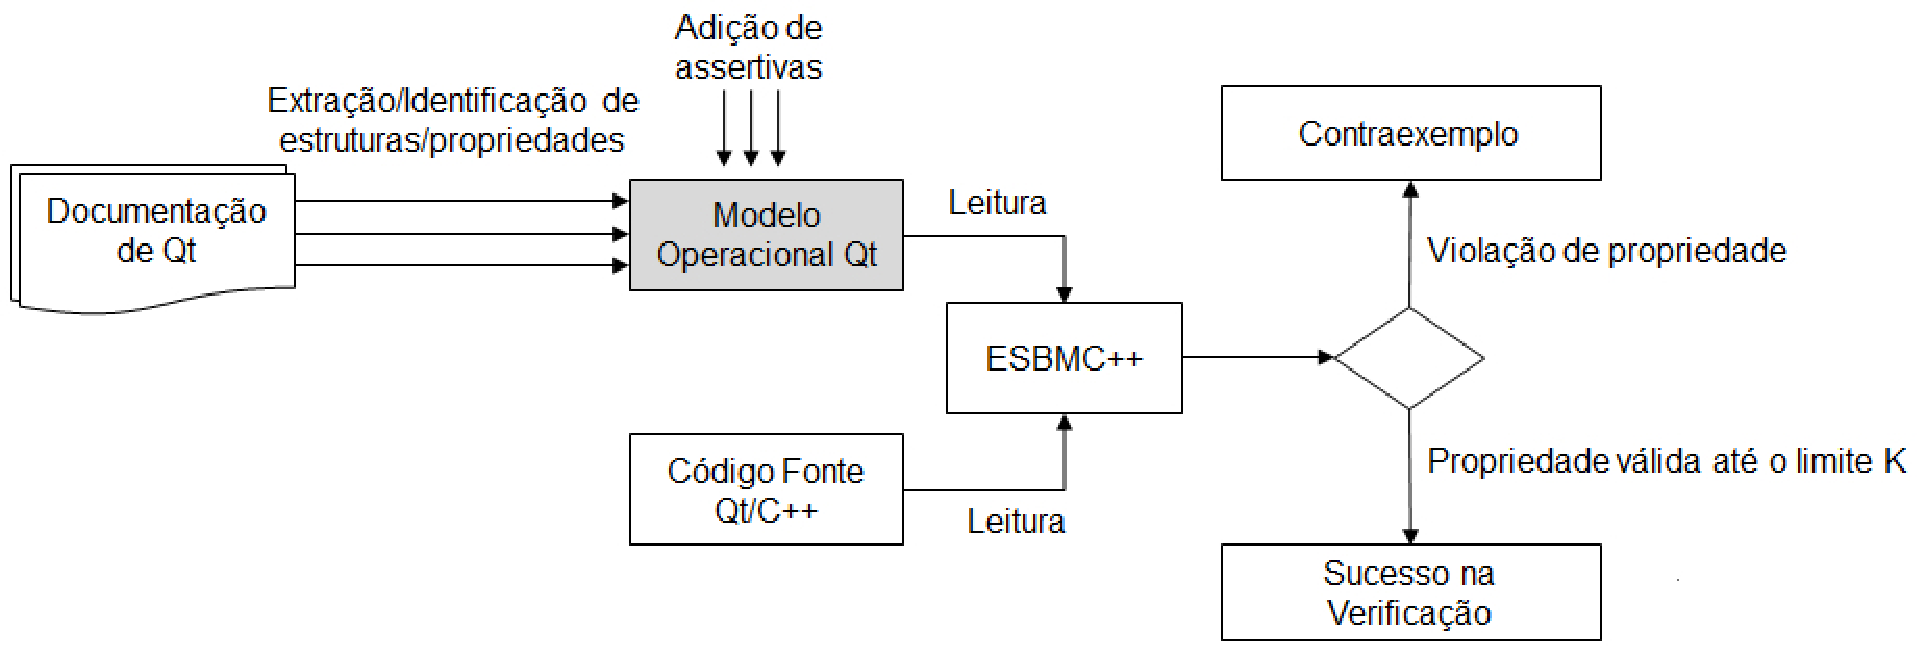
\includegraphics[width=5.5in]{figuras/Fig2.pdf}
  \caption{Conectando QtOM a ESBMC$++$.}
  \label{figure:Fig2}
\end{figure}


O m�dulo \textit{Qt Core} possui um subconjunto de classes denominado \textit{Qt Container}~\cite{Qt15} como alternativa para os \textit{containers} da \textit{Standard Template Library} (STL) dispon�veis na linguagem C++~\cite{Iso2003}. Por exemplo, durante o desenvolvimento de uma determinada aplica��o, � necess�rio a cria��o de uma pilha de tamanho vari�vel para o armazenamento de objetos do tipo \textit{QWidgets}, neste caso, uma alternativa seria o uso da classe \textit{QStack} que implementa um \textit{container} com a pol�tica LIFO (do ingl�s, \textit{last-in, first-out}) (\textit{e.g.}, \textit{QStack}$<$\textit{QWidget}$>$). Al�m disso, tais \textit{containers} tamb�m fazem uso de estruturas denominadas \textit{iterators} no estilo Java/STL, de modo a se deslocar ao longo dos dados armazenados no \textit{container} criado.  

Desta forma, esse subconjunto de classes pode ser classificado em dois subgrupos: sequenciais e associativos, dependendo da estrutura de armazenamento implementada. Neste contexto, as classes \textit{QList}, \textit{QLinkedList}, \textit{QVector}, \textit{QStack} e \textit{QQueue} s�o classificadas como \textit{containers} sequenciais, enquanto as classes \textit{QMap}, \textit{QMultiMap}, \textit{QHash}, \textit{QMultiHash} e \textit{QSet} s�o classificadas como \textit{containers} associativos.


\newpage

%%%%%%%%%%%%%%%%%%%%%%%%%%%%%%%%%%%%%%%%%%%%%%
\section{Pr�-condi��es}
\label{sec:preconditions}
%%%%%%%%%%%%%%%%%%%%%%%%%%%%%%%%%%%%%%%%%%%%%%

Ao se utilizar modelos limitados � poss�vel diminuir a complexidade que � associada as �rvores IRep. Desta forma, o ESBMC$++$ � capaz de construir �rvores IRep de uma forma muito r�pida, com baixa complexidade, mas que englobam todas as propriedades necess�rias para a verifica��o dos programas desejados. Al�m disso, o uso de assertivas se torna indispens�vel para verificar propriedades relacionadas aos m�todos do \textit{framework} multiplataforma Qt, assim como, as suas respectivas execu��es que n�o s�o contempladas pelas bibliotecas padr�es. Deste modo, tais assertivas s�o integrados aos respectivos m�todos com o objetivo de detectar viola��es em rela��o ao uso incorreto do framework Qt. 

Em resumo, baseado na adi��o de assertivas, ESBMC$++$ � capaz de verificar propriedades espec�ficas contidas em QtOM e identificar como pr�-condi��es partes das propriedades relacionadas, ou seja, as propriedades que devem ser mantidas de forma que haja uma execu��o correta de um determinado m�todo ou fun��o. Por exemplo, a abordagem proposta pode verificar se um par�metro, que representa uma determinada posi��o dentro de uma vetor � maior ou igual a zero.

De acordo com o fragmento de c�digo mostrado na Figura~\ref{fig:Fig3} que pertence a aplica��o chamada \textit{GeoMessage Simulator}. Esta aplica��o fornece mensagens para componentes do sistema na plataforma ArcGIS~\cite{geomessage}. Como mostrado, o m�todo $setFileName$() manipula uma pr�-condi��o (veja linha $6$), onde $m\_inputFile$ � um objeto da classe \textit{QFile} que proporciona uma interface de leitura e escrita para se manipular arquivos~\cite{Qt15}. Ao ser definido um nome ao arquivo, o objeto $fileName$ da \textit{QString} n�o pode ser nulo. Desta forma, quando $setFileName$() � chamado, o ESBMC$++$ interpreta o seu comportamento de acordo com o implementado em QtOM como mostrado na Figura~\ref{fig:Fig4}.

\begin{figure}[htb]
\centering
\begin{minipage}{0.6\textwidth}
\begin{lstlisting}
QString loadSimulationFile( const QString &fileName )
{
   if(m_inputFile.isOpen())
     m_inputFile.close();
     
   m_inputFile.setFileName(fileName);
   
   //Check file for at least one message
   if( !doInitialRead() ) 
   {
      return QString(m_inputFile.fileName() + "is an empty message file");
   }
   else
   {
      return NULL;
   }
}
\end{lstlisting}
\end{minipage}
\caption{Fragmento de c�digo da fun��o \textit{loadSimulationFile} presente no benchmark Geomessage Simulator.}
\label{fig:Fig3}
\end{figure}

A Figura~\ref{fig:Fig4} mostra um trecho do modelo operacional correspondente � classe QFile com uma implementa��o de $setFileName$() (veja as linhas 5-10), onde apenas as pr�-condi��es s�o verificadas. Em particular, se o objeto QString passado como um par�metro n�o estiver vazio (veja a linha 6), a opera��o � v�lida e, consequentemente, a premissa assumida � considerada \textit{verdadeira}. Caso contr�rio, se uma opera��o incorreta for realizada, como uma \textit{string} vazia for passada como par�metro, a premissa assumida � considerada \textit{falsa}. Nesse caso, o ESBMC$++$ retornaria um contraexemplo com todos os passos necess�rios para reproduzir a execu��o de tal viola��o, al�m de descrever o erro da respectiva premissa violada.\\


\begin{figure}[htb]
\centering
\begin{minipage}{0.5\textwidth}
\begin{lstlisting}
class QFile {
...
    QFile( const QString &name ) { ... }
    ...
    void setFileName( const QString &name ){
       __ESBMC_assert( !name.isEmpty(), "The string must not be empty" );
       __ESBMC_assert( !this->isOpen(), "The file must be closed" );
    }
    ...
};
\end{lstlisting}
\end{minipage}
\caption{Modelo operacional de $setFileName$() presente na classe QFile.}
\label{fig:Fig4}
\end{figure}

Do ponto de vista da verifica��o de software, existem m�todos/fun��es que tamb�m n�o apresentam qualquer propriedade a ser verificada como aqueles cuja �nica finalidade � imprimir valores na tela. Dado que ESBMC$++$ realiza o processo verifica��o a n�vel de software ao inv�s de testar o hardware, a corretude a cerca do valor impresso na tela n�o foi abordado neste trabalho. Por fim, para tais m�todos s� existem assinaturas, de modo que o verificador proposto seja capaz de reconhecer a estrutura desejada para que durante o processo de an�lise seja constru�do uma �rvores IRep confi�vel. No entanto, eles n�o apresentam qualquer modelagem (corpo de fun��o), uma vez que n�o exista nenhuma propriedade a n�vel de software a ser verificada.

%%%%%%%%%%%%%%%%%%%%%%%%%%%%%%%%%%%%%%%%%%%%%%
\section{P�s-condi��es}
\label{sec:postconditions}
%%%%%%%%%%%%%%%%%%%%%%%%%%%%%%%%%%%%%%%%%%%%%%

Em aplica��es reais existem m�todos que n�o cont�m apenas propriedades que ser�o tratadas como pr�-condi��o, mas tambem ser�o considerados como p�s-condi��es~\cite{monteiro2015,Musuvathi2002}. Por exemplo, de acordo com a documenta��o do Qt~\cite{Qt15}, a fun��o $setFileName$ conforme descrita na Se��o~\ref{sec:preconditions} n�o deve ser utilizada se o respectivo arquivo j� estiver sendo utilizado, o que � verificado em seu c�digo fonte a partir da estrutura $if$ presente nas linhas $3$ e $4$ visto na Figura~\ref{fig:Fig3}.

No entanto, a execu��o da instru��o presente na linha $4$ (veja Fig.~\ref{fig:Fig3}) seria n�o determin�stica para o ESBMC$++$, assim como, a assertiva presente na linha $8$ do modelo operacional associado, como mostrado na Figura~\ref{fig:Fig4}, uma vez que n�o h� como se afirmar se o respectivo arquivo est� sendo utilizado ou n�o. Desta forma, � evidente que ser� necess�rio simular o comportamento do m�todo $isOpen$() com o intuito de verificar de forma coerente as propriedades relacionadas com manipula��o de arquivos. Como a classe \textit{QFile} indiretamente herda os m�todos $open$() e $isOpen$(), a partir da classe \textit{QIODevice}, para simula��es comportamentais desses m�todos constr�i-se um modelo operacional para \textit{QIODevice} conforme mostrado na Figura~\ref{fig:Fig5}.

\begin{figure}[htb]
\centering
\begin{minipage}{0.47\textwidth}
\begin{lstlisting}
class QIODevice {
    ...
    bool QIODevice::open(OpenMode mode){
       this->__openMode = mode;
       if (this->__openMode == NotOpen)
           this->__isOpen = false;
       this->__isOpen = true;
    }
    
    bool isOpen() const{
       return this->__isOpen;
    }
    ...
private:
    bool __isOpen;
    OpenMode __openMode;
    ...
};
\end{lstlisting}
\end{minipage}
\caption{Modelo operacional para os m�todos $open$() e $isOpen$() na classe \textit{QIODevice}.}
\label{fig:Fig5}
\end{figure}

Por fim, todos os m�todos que resultam em uma condi��o que deve ser mantida, a fim de permitir uma adequada execu��o de futuras instru��es, devem apresentar uma simula��o do seu comportamento. Consequentemente, um determinado modelo operacional deve seguir de forma rigorosa as especifica��es descritas na documenta��o oficial do \textit{framework}~\cite{Qt15} com o objetivo de se obter o mesmo comportamento, assim como, incluir mecanismos necess�rios � verifica��o do c�digo. Como resultado, � necess�rio verificar o n�vel de equival�ncia entre o modelo operacional e a biblioteca original, com o intuito de se comparar o comportamento de ambos, tendo em vista que os modelos operacionais desenvolvidos s�o uma c�pia simplificada das bibliotecas originais com todos os mecanismos necess�rios para a verifica��o do c�digo~\cite{pereira2016}.

%%%%%%%%%%%%%%%%%%%%%%%%%%%%%%%%%%%%%%%%%%%%%%
\section{Linguagem Base}
\label{sec:language}
%%%%%%%%%%%%%%%%%%%%%%%%%%%%%%%%%%%%%%%%%%%%%%

Com o intuito de implementar o modelo operacional para as classes que comp�e o \textit{Qt Container}, a formaliza��o da linguagem base descrita por Ramalho \textit{et al.}~\cite{ECBS13} � utilizada e se estende at� a formula��o das propriedades $\mathcal{C}$ e $\mathcal{P}$. Contudo, tal linguagem foi adaptada, neste trabalho, com o objetivo de formular adequadamente a verifica��o de ambos tipos de \textit{containers} (\textit{i.e.}, sequencial ou associativo) como mostrado na Figura~\ref{ccl-fig}.  

\begin{figure}[htb]
\[\begin{array}{r@{\:\:}r@{\:\:}l}
  V  & ::= &
    v \:|\: \mathit{I_v} \:|\: \mathit{P_v}
\\[0.5ex]
  K  & ::= &
    k \:|\: \mathit{I_k} \:|\: \mathit{P_k}
\\[0.5ex]
   \mathit{I} & ::= &
     i \:|\: \mathit{C.begin()} \:|\: \mathit{C.end()}
\\  & | &
     \mathit{C.insert(\mathit{I}, \mathit{V}, \mathbb{N})} \:|\: \mathit{C.erase(\mathit{I})} \:|\: \mathit{C.search(\mathit{V})}
\\  & | &
     \mathit{C.insert(\mathit{K}, \mathit{V})} \:|\: \mathit{C.search(\mathit{K})}
\\[0.5ex]
   P  & ::= &
     p \:|\: P (+ \:|\: - ) P
       \:|\: \mathit{C_k} \:|\: \mathit{C_v} \:|\: \mathit{I_k} \:|\: \mathit{I_v}
\\[0.5ex]
   C  & ::= &
     c 
\\[0.5ex]
  \mathbb{N}  & ::= &
     n \:|\: \mathbb{N} (+ \:|\: * | \ldots) \mathbb{N}
       \:|\: \mathit{I_{pos}}
       \:|\: \mathit{C_{size}}
  \end{array}
\]
  \caption{Sintaxe da linguagem adaptada, base para a descri��o formal dos \textit{containers}.}
  \label{ccl-fig}
\end{figure}

De acordo com a Figura~\ref{ccl-fig}, os elementos b�sicos est�o divididos em dois dom�nios sint�ticos: $\mathit{V}$ para valores e $\mathit{K}$ para as chaves. No entanto, os demais dom�nios, $\mathit{I}$, $\mathit{P}$, $\mathbb{N}$ e $\mathit{C}$ s�o mantidos por \textit{iterators}, ponteiros, �ndices inteiros e express�es \textit{container} adequadas, respectivamente. Assim, as vari�veis $\mathit{k}$ do tipo $\mathit{K}$ e $\mathit{v}$ do tipo $\mathit{V}$ s�o adicionadas. Dessa forma, a nota��o $\mathit{I_v}$ representa um valor armazenado em um \textit{container} em uma posi��o direcionada pelo \textit{iterator} $\mathit{I}$ e $\mathit{I_k}$ representa uma chave armazenada em um \textit{container} em uma posi��o direcionada tamb�m pelo \textit{iterator} $\mathit{I}$. Tais nota��es s�o abrevia��es para $\mathit{store(i,I_{pos},I_v)}$ e $\mathit{store(i,I_{pos},I_k)}$, respectivamente, onde a express�o $\mathit{store}(t, f, v)$ indica \textit{container} $t$ que no campo $f$ possui um valor $v$. Da forma similar, $\mathit{P_k}$ e $\mathit{P_v}$ representam ponteiros para a chave e o valor, respectivamente.

Al�m disso, tr�s outros m�todos foram inclu�dos com o objetivo de descrever as opera��es realizadas em cada \textit{container}. O m�todo $\mathit{C.insert(k, v)}$ insere um valor $\mathit{v}$ no \textit{container} $C$ com uma chave correspondente $\mathit{k}$ e possui como retorno um \textit{iterator} que aponta para o novo elemento inserido. O m�todo $\mathit{C.search(k)}$ retorna um \textit{iterator} que aponta para a primeira evid�ncia de um elemento com uma chave $\mathit{k}$ correspondente. De modo semelhante, $\mathit{C.search(v)}$ tamb�m retorna um \textit{iterator} que aponta para a primeira evid�ncia de um elemento com um valor $\mathit{v}$ correspondente. No entanto, caso n�o exista nenhuma chave ou valor correspondente durante a opera��o com tais m�todos, os mesmos retornar�o $\mathit{C.end()}$, o qual corresponde ao \textit{iterator} que aponta para a posi��o imediatamente posterior ao �ltimo elemento. Por fim, $\mathit{C_k}$ � um endere�o de mem�ria que armazena o in�cio das chaves dos \textit{containers}, assim como, $\mathit{C_v}$ � usado para armazenar os valores dos \textit{containers}.

� importante ressaltar que, todas demais opera��es provenientes da linguagem base mencionada s�o utilizadas aqui de acordo como descrito por Ramalho \textit{et al.}~\cite{ECBS13}.

%%%%%%%%%%%%%%%%%%%%%%%%%%%%%%%%%%%%%%%%%%%%%%
\section{\textit{Containers} sequenciais}
\label{sec:sequential}
%%%%%%%%%%%%%%%%%%%%%%%%%%%%%%%%%%%%%%%%%%%%%%

\textit{Containers} sequenciais tem como objetivo armazenar elementos em uma determinada ordem~\cite{Deitel}. De acordo com a documenta��o do Qt~\cite{Qt15}, \textit{QList} � a classe \textit{container} mais utilizada e possui uma estrutura em formato de lista encadeada. Da mesma forma, \textit{QLinkedList} tamb�m possui um estrutura em forma de lista, embora seja acessada atrav�s de \textit{iterators} ao inv�s de �ndices inteiros. Na classe \textit{QVector}, h� presente uma estrutura de \textit{array} expans�vel e, por fim, \textit{QStack} e \textit{QQueue} fornecem estruturas que implementam diretivas como LIFO e FIFO (em ingl�s, \textit{first-in, first-out}), respectivamente.

Para simular adequadamente os \textit{containers} sequenciais, os modelos propostos utilizam da linguagem base descrita na Se��o~\ref{sec:language}. Os \textit{containers} sequenciais s�o implementados a partir de um ponteiro $\mathit{C_v}$ para os valores do \textit{container} e tamb�m com um $\mathit{C_{size}}$, o qual � utilizado para representar o tamanho do respectivo \textit{container} (onde $\mathit{C_{size}} \in \mathbb{N}$). Dessa forma, os \textit{iterators} s�o modelados por meio de duas vari�veis, uma do tipo $\mathbb{N}$ que � denominada de $\mathit{i_{pos}}$ e cont�m o valor do �ndice apontado por um \textit{iterator} e outra do tipo $P$ que � chamado por $\mathit{I_v}$ e aponta para um \textit{container} subjacente.

Vale ressaltar que todos os m�todos, a partir dessas bibliotecas, podem ser expressos em varia��es simplificadas de tr�s opera��es principais, \textit{insertion}($\mathit{C.insert(\mathit{I}, \mathit{V}, \mathbb{N})}$), \textit{deletion}($\mathit{C.erase(\mathit{I})}$) e \textit{\textit{search}}($\mathit{C.search(\mathit{V})}$). A partir da transforma��o SSA, os efeitos adversos sobre \textit{iterators} e \textit{containers} s�o expl�citos para que as opera��es retornem novos \textit{iterators} e \textit{containers}.

Por exemplo, um \textit{container} $c$ com uma chamada \textit{c.search}($v$) representa uma pesquisa pelo elemento $v$ no respectivo \textit{container}. Deste modo, se esse elemento for encontrado, � retornado um \textit{iterator} que aponta para o respectivo elemento, caso contr�rio, � retornado um \textit{iterator} que aponta para a posi��o imediatamente posterior ao �ltimo elemento do \textit{container} (\textit{i.e.}, $\mathit{c.end()}$). Desta forma, a instru��o ``$\mathit{c.search}(v);$'' torna-se ``$(c',i')=\mathit{c.search}(v);$'' que possuem efeitos adversos de forma expl�cita. Assim, a fun��o de tradu��o $\mathcal{C}$ descreve premissas que est�o relacionadas com o ``antes" e o ``depois" das respectivas vers�es das vari�veis do modelo. Na verdade, nota��es com ap�strofe (\textit{e.g.}, $c'$ and $i'$) representam o estado das vari�veis do modelo, ap�s realizar a execu��o da respectiva opera��o; nota��es simplificadas (\textit{e.g.}, $c$ and $i$) representam os estados anteriores. Al�m disso, $select(c, i = lower_{bound} \ldots i = upper_{bound})$ representa uma express�o de \textit{loop} (\textit{e.g.}, $for$ e $while$), onde cada valor de $c$, a partir da posi��o $lower_{bound}$ at� $upper_{bound}$, ser� selecionado. Da mesma forma, $store(c_{1}, lower_{bound}^{1},select(c_{2},lower_{bound}^{2}))$\\$ \ldots store(c_{1},upper_{bound}^{1},select(c_{2},upper_{bound}^{2}))$ tamb�m representa uma express�o de \textit{loop}, onde cada valor de $c_{2}$, a partir de posi��o $lower_{bound}^{2}$ at� a posi��o $upper_{bound}^{2}$ ser�o armazenados em $c_{1}$ nas posi��es $lower_{bound}^{1}$ at� $upper_{bound}^{1}$, respectivamente. Sendo assim,
%
\[\begin{array}{lll}
\multicolumn{3}{l}{{\mathcal{C}}((c',i')=c\mathit{.search}(v)):=}\\
  & \multicolumn{2}{l}{\wedge\:i' := c.\textit{begin}()}\\
  & \wedge\: g_0 := &\!\!\!\!\textit{select}(c_v, i_{pos} = 0 \ldots i_{pos} = c_{size} - 1) == v \\
%  & & \textit{select}(\ldots(\textit{select}(c_v, i_{pos} = 0),\\
%  & & \:\:\:\:\:\:\ldots,\\
%  & & i_{pos} = c_{size} - 1))) == v \\
  & \multicolumn{2}{l}{\wedge\:{i'}_{pos} := \textit{ite}(g_0, i_{pos}, c_{size})}\\
  & \multicolumn{2}{l}{\wedge\:{i'}_v := {c'}_v.}\\
\end{array}\]

Com rela��o aos \textit{containers} sequenciais, os m�todos $\mathit{C.insert(\mathit{I}, \mathit{V}, \mathbb{N})}$ e $\mathit{C.erase(\mathit{I})}$ se comportam como descrito por Ramalho \textit{et al.}~\cite{ECBS13}.

%%%%%%%%%%%%%%%%%%%%%%%%%%%%%%%%%%%%%%%%%%%%%%
\section{\textit{Containers} Associativos}
\label{sec:associative}
%%%%%%%%%%%%%%%%%%%%%%%%%%%%%%%%%%%%%%%%%%%%%%

O grupo dos \textit{containers} associativos possui cinco classes: \textit{QMap}, \textit{QMultimap}, \textit{QHash}, \textit{QMultiHash} e \textit{QSet}. \textit{QMap} tem como abordagem um vetor associativo que conecta cada umas das chaves, de um certo tipo $K$, a um valor de um certo tipo $V$, onde as chaves associadas s�o armazenadas em ordem. Por um lado, \textit{QHash} apresenta um comportamento similar ao \textit{QMap}, contudo os dados armazenados possuem uma ordem arbitr�ria. \textit{QMultiMap} e \textit{QMultihash} representam respectivamente subclasses de \textit{QMap} e \textit{QHash}, no entanto, ambas classes permitem o armazenamento de valores replicados. Por fim, \textit{QSet} armazena objetos que est�o associados a um conjunto de valores ordenados.

Com o intuito de implementar \textit{containers} associativos, um ponteiro $c_v$ � definido para os valores armazenados, um ponteiro $c_k$ � utilizado para armazenar as chaves do respectivo \textit{container} e uma vari�vel $c_{size}$ � utilizada para guardar a quantidade de elementos inseridos. Em especial, $c_k$ e $c_v$ est�o conectados por meio de um �ndice, ou seja, dado um \textit{container} $c$ que cont�m uma chave $k$ e um valor $v$ assume-se que

\[\begin{array}{r@{\:\:}c@{\:\:}l}
\left[\forall \omega \in \mathbb{N} | 0 \leq \omega < c_{size}\right]
\end{array}
\]

\noindent e

\[\begin{array}{r@{\:\:}c@{\:\:}l}
k \rightarrow v \iff select\left(c_k,\omega\right) = k \wedge select\left(c_v,\omega\right) = v,
\end{array}
\]

\noindent onde $(k \rightarrow v)$ indica que uma chave $k$ � associada a um valor $v$ and $\omega$ representa uma posi��o v�lida em $c_k$ e $c_v$. Al�m disso, a fun��o \emph{select(a, i)} indica o valor de $a$ em um �ndice $i$~\cite{ECBS13}. Novamente, todas as opera��es dessas bibliotecas podem ser expressadas a partir de uma varia��o simplificada das tr�s principais opera��es citadas na Se��o~\ref{sec:sequential}.

Portanto, a opera��o de inser��o para \textit{containers} associativos pode ser realizada de duas maneiras diferentes. Em primeiro lugar, se a ordem n�o importa, um novo elemento � inserido no final de $c_k$ e $c_v$. Desta forma, dado um container $c$, o m�todo $c.insert(k,v)$ ao ser chamado realiza inser��es de elementos no \textit{container} $c$ com um o valor $v$ e associado a uma chave $k$, por�m se $k$ j� existe, ele substitui o valor associado a $k$ por $v$ e retorna um \textit{iterator} que aponta para o elemento inserido ou modificado. Deste modo,
%
\[\begin{array}{lll}
\multicolumn{3}{l}{{\mathcal{C}}((c',i')=c\mathit{.insert}(k,v)):=}\\
  & \multicolumn{2}{l}{\wedge\:{c'}_{size} := {c}_{size} + 1}\\
  & \multicolumn{2}{l}{\wedge\:i' := c.\textit{begin}()}\\
  & \wedge\: g_0 := &\!\!\!\!\textit{select}(c_k, i_{pos} = 0 \ldots i_{pos} = c_{size} - 1) == k \\
  %& \wedge\: g_0 := &\!\!\!\!(\textit{select}(\ldots(\textit{select}(\\
  %& & \textit{select}(\ldots(\textit{select}(c_k, i_{pos} = 0),\\
  %& & \:\:\:\:\:\:\ldots,\\
  %& & i_{pos} = c_{size} - 1))) = k \\
  & \multicolumn{2}{l}{\wedge\:{i'}_{pos} := \textit{ite}(g_0, i_{pos}, c_{size})}\\
  & \wedge\: {c'}_k := &\!\!\!\!\textit{store}(c_k,{i'}_{pos} + 1, \textit{select}(c_k, {i'}_{pos})),\\
  & & \:\:\:\:\:\:\ldots,\\
  & & \textit{store}(c_k, c_{size}, \textit{select}(c_k, c_{size} - 1)))\\
  %& \wedge\: {c'}_k := &\!\!\!\!\textit{store}(\ldots(\textit{store}(c_k\\
  %& & {i'}_{pos} + 1, \textit{select}(c_k, {i'}_{pos})),\\
  %& & \:\:\:\:\:\:\ldots,\\
  %& & c_{size}, \textit{select}(c_k, c_{size} - 1)))\\
  & \wedge\: {c'}_v := &\!\!\!\!\textit{store}(c_v,{i'}_{pos} + 1, \textit{select}(c_v, {i'}_{pos})),\\
  & & \:\:\:\:\:\:\ldots,\\
  & & \textit{store}(c_v, c_{size}, \textit{select}(c_v, c_{size} - 1)))\\
  %& \wedge\: {c'}_v := &\!\!\!\!\textit{store}(\ldots(\textit{store}(c_v\\
  %& & {i'}_{pos} + 1, \textit{select}(c_v, {i'}_{pos})),\\
  %& & \:\:\:\:\:\:\ldots,\\
  %& & c_{size}, \textit{select}(c_v, c_{size} - 1)))\\
  & \multicolumn{2}{l}{\wedge\:{c'}_k := \textit{store}(c_k, {i'}_{pos}, k)}\\
  & \multicolumn{2}{l}{\wedge\:{c'}_v := \textit{store}(c_v, {i'}_{pos}, v)}\\
  & \multicolumn{2}{l}{\wedge\:{i'}_k := {c'}_k}\\
  & \multicolumn{2}{l}{\wedge\:{i'}_v := {c'}_v.}\\
\end{array}\]
%

Em uma outra vers�o do m�todo de inser��o onde a ordem das chaves possuem import�ncia. Todas as vari�veis citadas acima s�o consideradas e uma compara��o � realizada, a fim de assegurar que o novo elemento � inserido na ordem desejada. Assim,

%
\[\begin{array}{lll}
\multicolumn{3}{l}{{\mathcal{C}}((c',i')=c\mathit{.insert}(k,v)):=}\\
  & \multicolumn{2}{l}{\wedge\:{c'}_{size} := {c}_{size} + 1}\\
  & \multicolumn{2}{l}{\wedge\:i' := c.\textit{begin}()}\\
  & \wedge\: g_0 := &\!\!\!\!\textit{select}(c_k, i_{pos} = 0 \ldots i_{pos} = c_{size} - 1) > k \\
  & \wedge\: g_1 := &\!\!\!\!\textit{select}(c_k, i_{pos} = 0 \ldots i_{pos} = c_{size} - 1) == k \\
  & \multicolumn{2}{l}{\wedge\:{i'}_{pos} := \textit{ite}(g_0 \vee g_1, i_{pos}, c_{size})}\\
  & \wedge\: {c'}_k := &\!\!\!\!\textit{store}(c_k,{i'}_{pos} + 1, \textit{select}(c_k, {i'}_{pos})),\\
  & & \:\:\:\:\:\:\ldots,\\
  & & \textit{store}(c_k, c_{size}, \textit{select}(c_k, c_{size} - 1)))\\
  & \wedge\: {c'}_v := &\!\!\!\!\textit{store}(c_v,{i'}_{pos} + 1, \textit{select}(c_v, {i'}_{pos})),\\
  & & \:\:\:\:\:\:\ldots,\\
  & & \textit{store}(c_v, c_{size}, \textit{select}(c_v, c_{size} - 1)))\\
  & \multicolumn{2}{l}{\wedge\:{c'}_k := \textit{store}(c_k, {i'}_{pos}, k)}\\
  & \multicolumn{2}{l}{\wedge\:{c'}_v := \textit{store}(c_v, {i'}_{pos}, v)}\\
  & \multicolumn{2}{l}{\wedge\:{i'}_k := {c'}_k}\\
  & \multicolumn{2}{l}{\wedge\:{i'}_v := {c'}_v.}\\
\end{array}\]
%

Em casos onde chaves com v�rios valores associados s�o permitidos, a compara��o feita ser� ignorada, caso seja verificado que j� existe um elemento associado a respectiva chave analisada. Por fim, com o prop�sito de realizar uma exclus�o, o m�todo apagar, o qual � representado por $erase$($i$) onde $i$ � um \textit{iterator} que aponta para o elemento a ser exclu�do. Isso exclui o elemento apontado por $i$, movendo para tr�s todos os elementos seguidos pelo elemento que foi exclu�do. Deste modo,
%
\[\begin{array}{lll}
\multicolumn{3}{l}{{\mathcal{C}}((c',i')=c\mathit{.erase}(i)):=}\\
  & \multicolumn{2}{l}{\wedge\:{c'}_{size} := {c}_{size} - 1}\\
  & \wedge\: {c'}_k := &\!\!\!\!\textit{store}(c_k,{i'}_{pos}, \textit{select}(c_k, {i'}_{pos} + 1)),\\
  & & \:\:\:\:\:\:\ldots,\\
  & & \textit{store}(c_k, c_{size} - 2, \textit{select}(c_k, c_{size} - 1)))\\
  & \wedge\: {c'}_v := &\!\!\!\!\textit{store}(c_v,{i'}_{pos}, \textit{select}(c_v, {i'}_{pos} + 1)),\\
  & & \:\:\:\:\:\:\ldots,\\
  & & \textit{store}(c_v, c_{size} - 2, \textit{select}(c_v, c_{size} - 1)))\\
  & \multicolumn{2}{l}{\wedge\:{i'}_k := {c'}_k}\\
  & \multicolumn{2}{l}{\wedge\:{i'}_v := {c'}_v}\\
  & \multicolumn{2}{l}{\wedge\:{i'}_{pos} := {i}_{pos} + 1.}\\
\end{array}\]
%

Nota-se que tais modelos induzem implicitamente duas propriedades principais que possuem o objetivo de executar de forma correta as opera��es j� mencionadas. A princ�pio a primeira propriedade se torna evidente quando $c_k$ e $c_v$ s�o considerados n�o vazios, isto �, $c_{size}$ tamb�m n�o � nulo para as opera��es de busca e exclus�o de elementos. A segunda propriedade se torna evidente quando $i$ � considerado um \textit{iterator} do respectivo \textit{container} referido, isto �, dado um \textit{container} $c$ com os ponteiros bases $c_k$ e $c_v$, $i_k = c_k$ e $i_v = c_v$ s�o mantidos.% Na verdade, estas e outras propriedades espec�ficas s�o tratadas em seus respectivos modelos operacionais conforme descrito no cap�tulo~\ref{chapter:smt-bmc}.

%%%%%%%%%%%%%%%%%%%%%%%%%%%%%%%%%%%%%%%%%%%%%%
\section{Resumo}
%%%%%%%%%%%%%%%%%%%%%%%%%%%%%%%%%%%%%%%%%%%%%%

\textcolor{red}{Necess�rio reler e reescrever essa se��o}

Neste cap�tulo, foi descrito como � realizado o processo de verifica��o com ESBMC$++$ junto com o modelo operacional proposto (QtOM) de acordo como mostrado na figura~\ref{figure:Fig2}, logo em seguida, � descrito como o modelo operacional proposto se utiliza de pr�-condi��es para identificar partes das propriedades relacionadas ao \textit{framework} multiplataforma Qt, para que um determinado m�todo ou fun��o seja executado de forma correta. Por fim, descreve-se como QtOM usa p�s-condi��es para garantir o mesmo comportamento de m�todos ou fun��es, a serem analisados, em rela��o ao apresentado nas bibliotecas originais do \textit{framework}~\cite{Qt15}. Como resultado, o conte�do apresentado nesse cap�tulo fornece todo o embasamento necess�rio para compreens�o da verifica��o de programas Qt/C$++$, utilizando o ESBMC$++$ como ferramenta base e um modelo operacional que utiliza pr� e p�s-condi��es para analisar o \textit{framework} em quest�o.

Neste cap�tulo, foi descrito o subconjunto denominado \textit{Qt Container} que est� integrado ao m�dulo \textit{Qt Core} do \textit{framework} multiplataforma Qt, sendo classificado em dois subgrupos: sequenciais e associativos, dependendo da estrutura de armazenamento implementada, logo em seguida, � descrito a linguaguem base formalizada por Ramalho \textit{et al.}~\cite{ECBS13}, mas adaptada com o objetivo de formular adequadamente a verifica��o de ambos tipos de \textit{containers} existentes. Por fim, os \textit{containers} sequenciais e associativos foram descritos de forma detalhada, a fim de ressaltar todos os met�dos que constituem essas bibliotecas assim como, a forma que est�o implementados a partir de uma transforma��o SSA realizada. Como resultado, o conte�do apresentado nesse cap�tulo fornece todo o embasamento necess�rio a cerca modelo operacional criado para \textit{Qt Container} usado em QtOM.
%%%%%%%%%%%%%%%%%%%%%%%%%%%%%%%%%%%%%%%%%%%%%%
\chapter{Modelo Operacional para \textit{containers}}
\label{chapter:container-model}
%%%%%%%%%%%%%%%%%%%%%%%%%%%%%%%%%%%%%%%%%%%%%%

O m�dulo \textit{Qt Core} possui um subconjunto de classes denominado \textit{Qt Container}~\cite{Qt15} como alternativa para os \textit{containers} da \textit{Standard Template Library} (STL) dispon�veis na linguagem C++~\cite{Iso2003}. Por exemplo, durante o desenvolvimento de uma determinada aplica��o, � necess�rio a cria��o de uma pilha de tamanho vari�vel para o armazenamento de objetos do tipo \textit{QWidgets}, neste caso, uma alternativa seria o uso da classe \textit{QStack} que implementa um \textit{container} com a pol�tica LIFO (do ingl�s, \textit{last-in, first-out}) (\textit{e.g.}, \textit{QStack}$<$\textit{QWidget}$>$). Al�m disso, tais \textit{containers} tamb�m fazem uso de estruturas denominadas \textit{iterators} no estilo Java/STL, de modo a se deslocar ao longo dos dados armazenados no \textit{container} criado.  

Desta forma, esse subconjunto de classes pode ser classificado em dois subgrupos: sequenciais e associativos, dependendo da estrutura de armazenamento implementada. Neste contexto, as classes \textit{QList}, \textit{QLinkedList}, \textit{QVector}, \textit{QStack} e \textit{QQueue} s�o classificadas como \textit{containers} sequenciais, enquanto as classes \textit{QMap}, \textit{QMultiMap}, \textit{QHash}, \textit{QMultiHash} e \textit{QSet} s�o classificadas como \textit{containers} associativos.

Por fim, uma linguagem base � proposta na Se��o~\ref{sec:language} com o objetivo de formalizar a implementa��o de cada \textit{container} e, em seguida, as Se��es~\ref{sec:sequential} e~\ref{sec:associative} descrevem as implementa��es formais para os \textit{containers} sequenciais e associativos, respectivamente.

%%%%%%%%%%%%%%%%%%%%%%%%%%%%%%%%%%%%%%%%%%%%%%
\section{Linguagem Base}
\label{sec:language}
%%%%%%%%%%%%%%%%%%%%%%%%%%%%%%%%%%%%%%%%%%%%%%

Com o intuito de implementar o modelo operacional para as classes que comp�e o \textit{Qt Container}, a formaliza��o da linguagem base descrita por Ramalho \textit{et al.}~\cite{ECBS13} � utilizada e se estende at� a formula��o das propriedades $\mathcal{C}$ e $\mathcal{P}$. Contudo, tal linguagem foi adaptada, neste trabalho, com o objetivo de formular adequadamente a verifica��o de ambos tipos de \textit{containers} (\textit{i.e.}, sequencial ou associativo) como mostrado na figura~\ref{ccl-fig}.  

\begin{figure}[htb]
\[\begin{array}{r@{\:\:}r@{\:\:}l}
  V  & ::= &
    v \:|\: \mathit{I_v} \:|\: \mathit{P_v}
\\[0.5ex]
  K  & ::= &
    k \:|\: \mathit{I_k} \:|\: \mathit{P_k}
\\[0.5ex]
   \mathit{I} & ::= &
     i \:|\: \mathit{C.begin()} \:|\: \mathit{C.end()}
\\  & | &
     \mathit{C.insert(\mathit{I}, \mathit{V}, \mathbb{N})} \:|\: \mathit{C.erase(\mathit{I})} \:|\: \mathit{C.search(\mathit{V})}
\\  & | &
     \mathit{C.insert(\mathit{K}, \mathit{V})} \:|\: \mathit{C.search(\mathit{K})}
\\[0.5ex]
   P  & ::= &
     p \:|\: P (+ \:|\: - ) P
       \:|\: \mathit{C_k} \:|\: \mathit{C_v} \:|\: \mathit{I_k} \:|\: \mathit{I_v}
\\[0.5ex]
   C  & ::= &
     c 
\\[0.5ex]
  \mathbb{N}  & ::= &
     n \:|\: \mathbb{N} (+ \:|\: * | \ldots) \mathbb{N}
       \:|\: \mathit{I_{pos}}
       \:|\: \mathit{C_{size}}
  \end{array}
\]
  \caption{Sintaxe da linguagem adaptada, base para a descri��o formal dos \textit{conatiners}.}
  \label{ccl-fig}
\end{figure}

De acordo com a figura acima, os elementos b�sicos est�o divididos em dois dom�nios sint�ticos: $\mathit{V}$ para valores e $\mathit{K}$ para as chaves. No entanto, os demais dom�nios, $\mathit{I}$, $\mathit{P}$, $\mathbb{N}$ e $\mathit{C}$ s�o mantidos por \textit{iterators}, ponteiros, �ndices inteiros e express�es \textit{container} adequadas, respectivamente. Assim, as vari�veis $\mathit{k}$ do tipo $\mathit{K}$ e $\mathit{v}$ do tipo $\mathit{V}$ s�o adicionadas. Dessa forma, a nota��o $\mathit{I_v}$ representa um valor armazenado em um \textit{container} em uma posi��o direcionada pelo \textit{iterator} $\mathit{I}$ e $\mathit{I_k}$ representa uma chave armazenada em um \textit{container} em uma posi��o direcionada tamb�m pelo \textit{iterator} $\mathit{I}$. Tais nota��es s�o abrevia��es para $\mathit{store(i,I_{pos},I_v)}$ e $\mathit{store(i,I_{pos},I_k)}$, respectivamente, onde a express�o $\mathit{store}(t, f, v)$ indica \textit{container} $t$ que no campo $f$ possui um valor $v$. Da forma similar, $\mathit{P_k}$ e $\mathit{P_v}$ representam ponteiros para a chave e o valor, respectivamente.

Al�m disso, tr�s outros m�todos foram inclu�dos com o objetivo de descrever as opera��es realizadas em cada \textit{container}. O m�todo $\mathit{C.insert(k, v)}$ insere um valor $\mathit{v}$ no \textit{container} $C$ com uma chave correspondente $\mathit{k}$ e possui como retorno um \textit{iterator} que aponta para o novo elemento inserido. O m�todo $\mathit{C.search(k)}$ retorna um \textit{iterator} que aponta para a primeira evid�ncia de um elemento com uma chave $\mathit{k}$ correspondente. De modo semelhante, $\mathit{C.search(v)}$ tamb�m retorna um \textit{iterator} que aponta para a primeira evid�ncia de um elemento com um valor $\mathit{v}$ correspondente. No entanto, caso n�o exista nenhuma chave ou valor correspondente durante a opera��o com tais m�todos, os mesmos retornar�o $\mathit{C.end()}$, o qual corresponde ao \textit{iterator} que aponta para a posi��o imediatamente posterior ao �ltimo elemento. Por fim, $\mathit{C_k}$ � um endere�o de mem�ria que armazena o in�cio das chaves dos \textit{containers}, assim como, $\mathit{C_v}$ � usado para armazenar os valores dos \textit{containers}.

� importante ressaltar que, todas demais opera��es provenientes da linguagem base mencionada s�o utilizadas aqui de acordo como descrito por Ramalho \textit{et al.}~\cite{ECBS13}.

%%%%%%%%%%%%%%%%%%%%%%%%%%%%%%%%%%%%%%%%%%%%%%
\section{\textit{Containers} sequenciais}
\label{sec:sequential}
%%%%%%%%%%%%%%%%%%%%%%%%%%%%%%%%%%%%%%%%%%%%%%

\textit{Containers} sequenciais tem como objetivo armazenar elementos em uma determinada ordem~\cite{Deitel}. De acordo com a documenta��o do Qt~\cite{Qt15}, \textit{QList} � a classe \textit{container} mais utilizada e possui uma estrutura em formato de lista encadeada. Da mesma forma, \textit{QLinkedList} tamb�m possui um estrutura em forma de lista, embora seja acessada atrav�s de \textit{iterators} ao inv�s de �ndices inteiros. Na classe \textit{QVector}, h� presente uma estrutura de \textit{array} expans�vel e, por fim, \textit{QStack} e \textit{QQueue} fornecem estruturas que implementam diretivas como LIFO e FIFO (em ingl�s, \textit{first-in, first-out}), respectivamente.

Para simular adequadamente os \textit{containers} sequenciais, os modelos propostos se utilizam da linguagem base descrita na se��o~\ref{sec:language}. Os \textit{containers} sequenciais s�o implementados a partir de um ponteiro $\mathit{C_v}$ para os valores do \textit{container} e tamb�m com um $\mathit{C_{size}}$, o qual � utilizado para representar o tamanho do respectivo \textit{container} (onde $\mathit{C_{size}} \in \mathbb{N}$). Dessa forma, os \textit{iterators} s�o modelados por meio de duas vari�veis, uma do tipo $\mathbb{N}$ que � denominada de $\mathit{i_{pos}}$ e cont�m o valor do �ndice apontado por um \textit{iterator} e outra do tipo $P$ que � chamado por $\mathit{I_v}$ e aponta para um \textit{container} subjacente.

Vale ressaltar que todos os m�todos, a partir dessas bibliotecas, podem ser expressos em varia��es simplificadas de tr�s opera��es principais, \textit{insertion}($\mathit{C.insert(\mathit{I}, \mathit{V}, \mathbb{N})}$), \textit{deletion}($\mathit{C.erase(\mathit{I})}$) e \textit{\textit{search}}($\mathit{C.search(\mathit{V})}$). A partir da transforma��o SSA, os efeitos adversos sobre \textit{iterators} e \textit{containers} s�o expl�citos para que as opera��es retornem novos \textit{iterators} e \textit{containers}.

Por exemplo, um \textit{container} $c$ com uma chamada \textit{c.search}($v$) representa uma pesquisa pelo elemento $v$ no respectivo \textit{container}. Deste modo, se esse elemento for encontrado, � retornado um \textit{iterator} que aponta para o respectivo elemento, caso contr�rio, � retornado um \textit{iterator} que aponta para a posi��o imediatamente posterior ao �ltimo elemento do \textit{container} (\textit{i.e.}, $\mathit{c.end()}$). Desta forma, a instru��o ``$\mathit{c.search}(v);$'' torna-se ``$(c',i')=\mathit{c.search}(v);$'' que possuem efeitos adversos de forma expl�cita. Assim, a fun��o de tradu��o $\cal C$ descreve premissas que est�o relacionadas com o ``antes" e o ``depois" das respectivas vers�es das vari�veis do modelo. Na verdade, nota��es com ap�strofe (\textit{e.g.}, $c'$ and $i'$) representam o estado das vari�veis do modelo, ap�s realizar a execu��o da respectiva opera��o; nota��es simplificadas (\textit{e.g.}, $c$ and $i$) representam os estados anteriores. Al�m disso, $select(c, i = lower_{bound} \ldots i = upper_{bound})$ representa uma express�o de \textit{loop} (\textit{e.g.}, $for$ e $while$), onde cada valor de $c$, a partir da posi��o $lower_{bound}$ at� $upper_{bound}$, ser� selecionado. Da mesma forma, $store(c_{1}, lower_{bound}^{1},select(c_{2},lower_{bound}^{2}))$\\$ \ldots store(c_{1},upper_{bound}^{1},select(c_{2},upper_{bound}^{2}))$ tamb�m representa uma express�o de \textit{loop}, onde cada valor de $c_{2}$, a partir de posi��o $lower_{bound}^{2}$ at� a posi��o $upper_{bound}^{2}$ ser�o armazenados em $c_{1}$ nas posi��es $lower_{bound}^{1}$ at� $upper_{bound}^{1}$, respectivamente. Sendo assim,
%
\[\begin{array}{lll}
\multicolumn{3}{l}{{\cal C}((c',i')=c\mathit{.search}(v)):=}\\
  & \multicolumn{2}{l}{\wedge\:i' := c.\textit{begin}()}\\
  & \wedge\: g_0 := &\!\!\!\!\textit{select}(c_v, i_{pos} = 0 \ldots i_{pos} = c_{size} - 1) == v \\
%  & & \textit{select}(\ldots(\textit{select}(c_v, i_{pos} = 0),\\
%  & & \:\:\:\:\:\:\ldots,\\
%  & & i_{pos} = c_{size} - 1))) == v \\
  & \multicolumn{2}{l}{\wedge\:{i'}_{pos} := \textit{ite}(g_0, i_{pos}, c_{size})}\\
  & \multicolumn{2}{l}{\wedge\:{i'}_v := {c'}_v.}\\
\end{array}\]

Com rela��o aos \textit{containers} sequenciais, os m�todos $\mathit{C.insert(\mathit{I}, \mathit{V}, \mathbb{N})}$ e $\mathit{C.erase(\mathit{I})}$ se comportam como descrito por Ramalho \textit{et al.}~\cite{ECBS13}.

%%%%%%%%%%%%%%%%%%%%%%%%%%%%%%%%%%%%%%%%%%%%%%
\section{\textit{Containers} Associativos}
\label{sec:associative}
%%%%%%%%%%%%%%%%%%%%%%%%%%%%%%%%%%%%%%%%%%%%%%

O grupo dos \textit{containers} associativos possui cinco classes: \textit{QMap}, \textit{QMultimap}, \textit{QHash}, \textit{QMultiHash} e \textit{QSet}. \textit{QMap} tem como abordagem um vetor associativo que conecta cada umas das chaves, de um certo tipo $K$, a um valor de um certo tipo $V$, onde as chaves associadas s�o armazenadas em ordem. Por um lado, \textit{QHash} apresenta um comportamento similar ao \textit{QMap}, contudo os dados armazenados possuem uma ordem arbitr�ria. \textit{QMultiMap} e \textit{QMultihash} representam respectivamente subclasses de \textit{QMap} e \textit{QHash}, no entanto, ambas classes permitem o armazenamento de valores replicados. Por fim, \textit{QSet} armazena objetos que est�o associados a um conjunto de valores ordenados.

Com o intuito de implementar \textit{containers} associativos, um ponteiro $c_v$ � definido para os valores armazenados, um ponteiro $c_k$ � utilizado para armazenar as chaves do respectivo \textit{container} e uma vari�vel $c_{size}$ � utilizada para guardar a quantidade de elementos inseridos. Em especial, $c_k$ e $c_v$ est�o conectados por meio de um �ndice, ou seja, dado um \textit{container} $c$ que cont�m uma chave $k$ e um valor $v$ assume-se que

\[\begin{array}{r@{\:\:}c@{\:\:}l}
\left[\forall \omega \in \mathbb{N} | 0 \leq \omega < c_{size}\right]
\end{array}
\]

\noindent e

\[\begin{array}{r@{\:\:}c@{\:\:}l}
k \rightarrow v \iff select\left(c_k,\omega\right) = k \wedge select\left(c_v,\omega\right) = v,
\end{array}
\]

\noindent onde $(k \rightarrow v)$ indica que uma chave $k$ � associada a um valor $v$ and $\omega$ representa uma posi��o v�lida em $c_k$ e $c_v$. Al�m disso, a fun��o \emph{select(a, i)} indica o valor de $a$ em um �ndice $i$~\cite{ECBS13}. Novamente, todas as opera��es dessas bibliotecas podem ser expressadas a partir de uma varia��o simplificada das tr�s principais opera��es citadas na Se��o~\ref{sec:sequential}.

Portanto, a opera��o de inser��o para \textit{containers} associativos pode ser realizada de duas maneiras diferentes. Em primeiro lugar, se a ordem n�o importa, um novo elemento � inserido no final de $c_k$ e $c_v$. Desta forma, dado um container $c$, o m�todo $c.insert(k,v)$ ao ser chamado realiza inser��es de elementos no \textit{container} $c$ com um o valor $v$ e associado a uma chave $k$, por�m se $k$ j� existe, ele substitui o valor associado a $k$ por $v$ e retorna um \textit{iterator} que aponta para o elemento inserido ou modificado. Deste modo,
%
\[\begin{array}{lll}
\multicolumn{3}{l}{{\cal C}((c',i')=c\mathit{.insert}(k,v)):=}\\
  & \multicolumn{2}{l}{\wedge\:{c'}_{size} := {c}_{size} + 1}\\
  & \multicolumn{2}{l}{\wedge\:i' := c.\textit{begin}()}\\
  & \wedge\: g_0 := &\!\!\!\!\textit{select}(c_k, i_{pos} = 0 \ldots i_{pos} = c_{size} - 1) == k \\
  %& \wedge\: g_0 := &\!\!\!\!(\textit{select}(\ldots(\textit{select}(\\
  %& & \textit{select}(\ldots(\textit{select}(c_k, i_{pos} = 0),\\
  %& & \:\:\:\:\:\:\ldots,\\
  %& & i_{pos} = c_{size} - 1))) = k \\
  & \multicolumn{2}{l}{\wedge\:{i'}_{pos} := \textit{ite}(g_0, i_{pos}, c_{size})}\\
  & \wedge\: {c'}_k := &\!\!\!\!\textit{store}(c_k,{i'}_{pos} + 1, \textit{select}(c_k, {i'}_{pos})),\\
  & & \:\:\:\:\:\:\ldots,\\
  & & \textit{store}(c_k, c_{size}, \textit{select}(c_k, c_{size} - 1)))\\
  %& \wedge\: {c'}_k := &\!\!\!\!\textit{store}(\ldots(\textit{store}(c_k\\
  %& & {i'}_{pos} + 1, \textit{select}(c_k, {i'}_{pos})),\\
  %& & \:\:\:\:\:\:\ldots,\\
  %& & c_{size}, \textit{select}(c_k, c_{size} - 1)))\\
  & \wedge\: {c'}_v := &\!\!\!\!\textit{store}(c_v,{i'}_{pos} + 1, \textit{select}(c_v, {i'}_{pos})),\\
  & & \:\:\:\:\:\:\ldots,\\
  & & \textit{store}(c_v, c_{size}, \textit{select}(c_v, c_{size} - 1)))\\
  %& \wedge\: {c'}_v := &\!\!\!\!\textit{store}(\ldots(\textit{store}(c_v\\
  %& & {i'}_{pos} + 1, \textit{select}(c_v, {i'}_{pos})),\\
  %& & \:\:\:\:\:\:\ldots,\\
  %& & c_{size}, \textit{select}(c_v, c_{size} - 1)))\\
  & \multicolumn{2}{l}{\wedge\:{c'}_k := \textit{store}(c_k, {i'}_{pos}, k)}\\
  & \multicolumn{2}{l}{\wedge\:{c'}_v := \textit{store}(c_v, {i'}_{pos}, v)}\\
  & \multicolumn{2}{l}{\wedge\:{i'}_k := {c'}_k}\\
  & \multicolumn{2}{l}{\wedge\:{i'}_v := {c'}_v.}\\
\end{array}\]
%

Em uma outra vers�o do m�todo de inser��o onde a ordem das chaves possuem import�ncia. Todas as vari�veis citadas acima s�o consideradas e uma compara��o � realizada, a fim de assegurar que o novo elemento � inserido na ordem desejada. Assim,

%
\[\begin{array}{lll}
\multicolumn{3}{l}{{\cal C}((c',i')=c\mathit{.insert}(k,v)):=}\\
  & \multicolumn{2}{l}{\wedge\:{c'}_{size} := {c}_{size} + 1}\\
  & \multicolumn{2}{l}{\wedge\:i' := c.\textit{begin}()}\\
  & \wedge\: g_0 := &\!\!\!\!\textit{select}(c_k, i_{pos} = 0 \ldots i_{pos} = c_{size} - 1) > k \\
  & \wedge\: g_1 := &\!\!\!\!\textit{select}(c_k, i_{pos} = 0 \ldots i_{pos} = c_{size} - 1) == k \\
  & \multicolumn{2}{l}{\wedge\:{i'}_{pos} := \textit{ite}(g_0 \vee g_1, i_{pos}, c_{size})}\\
  & \wedge\: {c'}_k := &\!\!\!\!\textit{store}(c_k,{i'}_{pos} + 1, \textit{select}(c_k, {i'}_{pos})),\\
  & & \:\:\:\:\:\:\ldots,\\
  & & \textit{store}(c_k, c_{size}, \textit{select}(c_k, c_{size} - 1)))\\
  & \wedge\: {c'}_v := &\!\!\!\!\textit{store}(c_v,{i'}_{pos} + 1, \textit{select}(c_v, {i'}_{pos})),\\
  & & \:\:\:\:\:\:\ldots,\\
  & & \textit{store}(c_v, c_{size}, \textit{select}(c_v, c_{size} - 1)))\\
  & \multicolumn{2}{l}{\wedge\:{c'}_k := \textit{store}(c_k, {i'}_{pos}, k)}\\
  & \multicolumn{2}{l}{\wedge\:{c'}_v := \textit{store}(c_v, {i'}_{pos}, v)}\\
  & \multicolumn{2}{l}{\wedge\:{i'}_k := {c'}_k}\\
  & \multicolumn{2}{l}{\wedge\:{i'}_v := {c'}_v.}\\
\end{array}\]
%

Em casos onde chaves com v�rios valores associados s�o permitidos, a compara��o feita ser� ignorada, caso seja verificado que j� existe um elemento associado a respectiva chave analisada. Por fim, com o prop�sito de realizar uma exclus�o, o m�todo apagar, o qual � representado por $erase$($i$) onde $i$ � um \textit{iterator} que aponta para o elemento a ser exclu�do. Isso exclui o elemento apontado por $i$, movendo para tr�s todos os elementos seguidos pelo elemento que foi exclu�do. Deste modo,
%
\[\begin{array}{lll}
\multicolumn{3}{l}{{\cal C}((c',i')=c\mathit{.erase}(i)):=}\\
  & \multicolumn{2}{l}{\wedge\:{c'}_{size} := {c}_{size} - 1}\\
  & \wedge\: {c'}_k := &\!\!\!\!\textit{store}(c_k,{i'}_{pos}, \textit{select}(c_k, {i'}_{pos} + 1)),\\
  & & \:\:\:\:\:\:\ldots,\\
  & & \textit{store}(c_k, c_{size} - 2, \textit{select}(c_k, c_{size} - 1)))\\
  & \wedge\: {c'}_v := &\!\!\!\!\textit{store}(c_v,{i'}_{pos}, \textit{select}(c_v, {i'}_{pos} + 1)),\\
  & & \:\:\:\:\:\:\ldots,\\
  & & \textit{store}(c_v, c_{size} - 2, \textit{select}(c_v, c_{size} - 1)))\\
  & \multicolumn{2}{l}{\wedge\:{i'}_k := {c'}_k}\\
  & \multicolumn{2}{l}{\wedge\:{i'}_v := {c'}_v}\\
  & \multicolumn{2}{l}{\wedge\:{i'}_{pos} := {i}_{pos} + 1.}\\
\end{array}\]
%

Nota-se que tais modelos induzem implicitamente duas propriedades principais que possuem o objetivo de executar de forma correta as opera��es j� mencionadas. A princ�pio a primeira propriedade se torna evidente quando $c_k$ e $c_v$ s�o considerados n�o vazios, isto �, $c_{size}$ tamb�m n�o � nulo para as opera��es de busca e exclus�o de elementos. A segunda propriedade se torna evidente quando $i$ � considerado um \textit{iterator} do respectivo \textit{container} referido, isto �, dado um \textit{container} $c$ com os ponteiros bases $c_k$ e $c_v$, $i_k = c_k$ e $i_v = c_v$ s�o mantidos. Na verdade, estas e outras propriedades espec�ficas s�o tratadas em seus respectivos modelos operacionais conforme descrito no cap�tulo~\ref{chapter:smt-bmc}.

%%%%%%%%%%%%%%%%%%%%%%%%%%%%%%%%%%%%%%%%%%%%%%
\section{Resumo}
%%%%%%%%%%%%%%%%%%%%%%%%%%%%%%%%%%%%%%%%%%%%%%

Neste cap�tulo, foi descrito o subconjunto denominado \textit{Qt Container} que est� integrado ao m�dulo \textit{Qt Core} do \textit{framework} multiplataforma Qt, sendo classificado em dois subgrupos: sequenciais e associativos, dependendo da estrutura de armazenamento implementada, logo em seguida, � descrito a linguaguem base formalizada por Ramalho \textit{et al.}~\cite{ECBS13}, mas adaptada com o objetivo de formular adequadamente a verifica��o de ambos tipos de \textit{containers} existentes. Por fim, os \textit{containers} sequenciais e associativos foram descritos de forma detalhada, a fim de ressaltar todos os met�dos que constituem essas bibliotecas assim como, a forma que est�o implementados a partir de uma transforma��o SSA realizada. Como resultado, o conte�do apresentado nesse cap�tulo fornece todo o embasamento necess�rio a cerca modelo operacional criado para \textit{Qt Container} usado em QtOM.


%Chama outro arquivo%
%%%%%%%%%%%%%%%%%%%%%%%%%%%%%%%%%%%%%%%%%%%%%%%
\section{\textit{Templates}}
\label{cpp-templates}
%%%%%%%%%%%%%%%%%%%%%%%%%%%%%%%%%%%%%%%%%%%%%%

Templates


%%%%%%%%%%%%%%%%%%%%%%%%%%%%%%%%%%%%%%%%%%%%%%
\chapter{Avalia��o experimental}
\label{sec:dis}
%%%%%%%%%%%%%%%%%%%%%%%%%%%%%%%%%%%%%%%%%%%%%%

Este cap�tulo � dividido em quatro partes. Se��o~\ref{sec:setup} descreve toda configura��o experimental utilizada, os experimentos e todos os par�metros de avalia��o utilizados para a realiza��o das avalia��es. Na Se��o~\ref{sec:benchmark}, a corretude e tamb�m o desempenho da metodologia proposta s�o verificados, utilizando programas Qt/C$++$ sequenciais baseados na documenta��o do \textit{framework} multiplataforma Qt~\cite{Qt15}. Na Se��o~\ref{sec:evaluation} � descrito os resultados obtidos a cerca da verifica��o de todos os casos de teste presentes na suite de teste \textit{esbmc--qt} utilizando ferramentas de verifica��o distintas (ESBMC$++$, LLBMC e DIVINE) com o objetivo de analisar a corretude e a efic�cia do modelo operacional proposto junto as ferramentas mencionadas. Por fim, � descrito na Se��o~\ref{sec:realqt} os resultados da verifica��o para as duas aplica��es reais (\textit{Locomaps}~\cite{locomaps} e \textit{GeoMessage Simulator}~\cite{geomessage}) utilizando o modelo operacional proposto denominado QtOM.

%%%%%%%%%%%%%%%%%%%%%%%%%%%%%%%%%%%%%%%%%%%%%%
\section{Configura��o dos Experimentos}
\label{sec:setup}
%%%%%%%%%%%%%%%%%%%%%%%%%%%%%%%%%%%%%%%%%%%%%%

Com o intuito de avaliar a efic�cia da abordagem proposta acerca da verifica��o de programas que utilizam o \textit{framework} Qt, foi criando um conjunto de testes autom�ticos denomidado \textit{esbmc--qt}. Em resumo, este conjunto de testes cont�m $711$ programas Qt/C$++$ ($12903$ linhas de c�digo), ou seja, todos os casos de teste utilizadas na atual avalia��o.

Os casos de teste mencionados acima est�o dividos em 10 principais conjuntos de teste, denominados QHash, QLinkedList, QList, QMap, QMultiHash, QMultiMap, QQueue, QSet, QStack e QVector. Vale ressaltar que todos os conjuntos de teste criados possuem casos de teste de acordo com a respectiva classe \textit{container} a ser analisada que em sua maioria possuem acesso aos m�dulos \textit{Qt Core} e \textit{Qt GUI} (\textit{e.g}, conjunto de teste QHash possui casos de testes que foram utilizados para avaliar o processo de verifica��o da classe \textit{container QHash} pertencente ao \textit{framework} multiplataforma Qt). Alguns casos de teste foram desenvolvidos a partir da documenta��o referente ao \textit{framework} analisado e os restantes foram desenvolvidos especificamente para analisar todas as caracter�stica fornecidas pelo \textit{framework}. Al�m disso, cada caso de teste � verificado manualmente antes de ser adicionado ao seu respectivo conjunto de teste. Desta forma, � capaz de se identificar se um determinado caso de teste possui ou n�o qualquer erro e est� de acordo com a opera��o a ser realizada. Assim, com base nesta revis�o, � poss�vel garantir que $353$ dos $711$ casos de teste cont�m erro (\textit{i.e.}, $49.65$\% do casos de teste analisados cont�m erro) e $358$ casos de teste n�o possuem falhas (\textit{i.e.}, $50.35$\% dos casos de teste analisados s�o considerados corretos). Na realidade esse tipo de revis�o � essencial para a avalia��o experimental, uma vez que pode-se comparar os resultados obtidos atrav�s da verifica��o realizada pelas ferramentas de verifica��o utilizadas e avaliar adequadamente se erros reais foram encontrados. 

Todos os experimentos foram realizados em um computador Intel Core $i7$-$4790$ com $3.60$ GHz de clock e $24$ GB ($22$ GB de mem�ria RAM e $2$ GB de m�moria virtual), utilizando-se um sistema operacional \textit{open source} de $64$ bits denominado Fedora. Al�m disso, tamb�m se utilizou a ferramenta de verifica��o ESBMC$++$~$v1.25.4$ com tr�s tipos de solucionadores SMT instalados (Z3~$v4.0$, Boolector~$v2.0.1$ e Yices 2~$v4.1$). Os limites de tempo e mem�ria utilizados para cada caso de teste foram definidos em 600 segundos e 22 GB, respectivamente. Por fim, uma avalia��o foi realizada utilizando o CBMC~$v5.1$, LLBMC~$v2013.1$ e DIVINE~$v3.3.2$ combinados com o modelo operacinal proposto (QtOM) com o objetivo de proporcionar compara��es entre ferramentas. Os per�odos de tempo foram indicados usando a fun��o \verb|clock_gettime| a partir da biblioteca \verb|time.h|~\cite{time}.

%%%%%%%%%%%%%%%%%%%%%%%%%%%%%%%%%%%%%%%%%%%%%%
\section{Compara��o entre solucionadores SMT}
\label{sec:benchmark}
%%%%%%%%%%%%%%%%%%%%%%%%%%%%%%%%%%%%%%%%%%%%%%

� conhecido que diferentes solucionadores SMT podem afetar fortemente os resultados obtidos~\cite{TSE12}, uma vez que n�o existe homogeneidade em rela��o a abordagem de implementa��o e respectivas heur�sticas. Primeiramente, as verifica��es que foram realizadas, utilizaram os tr�s solucionadores SMT j� mencionados (Z3, Boolector e Yices 2). Desta forma, Yices 2 obteve os piores resultados, apresentando uma taxa de cobertura de $78$\% e um tempo de verifica��o de $26,27$ minutos. Dessa forma, o Yices 2 n�o conseguiu resolver corretamente as f�rmulas SMT originadas do processo de verifica��o dos diversos casos de teste. Por outro lado, tanto os solucionadores Z3 quanto Boolector apresentaram uma taxa de cobertura de $89$\%, apesar do tempo de verifica��o obtido ao se realizar as verifica��es utilizando o solucionador Z3 seja inferior as realizadas com o solucionador Boolector, onde, respectivamente, s�o apresentados tempos de verifica��o de $223,6$ minutos e $26,38$ minutos. A partir dos resultados mencionados, o solucionador Boolector mostrou-se $8,5$ vezes mais r�pido do que o solucionador Z3, apesar da mesma precis�o de ambos, mas quatro casos de teste relataram viola��es a cerca do tempo limite determinado. Al�m disso, o Yices 2 n�o conseguiu analisar completamente todos os conjuntos de teste desenvolvidos, pois, n�o possui suporte a tuplas, logo, apresentou a menor taxa de cobertura e o menor tempo. Em resumo, de acordo com a Figura~\ref{figure:solver-comparison}, o Boolector se apresenta como o melhor solucionador para o processo de verifica��o proposto, pois apresenta em menor tempo a maior taxa de cobertura.

\begin{figure}[htb]
\centering
\subfloat[Taxa de cobertura]{
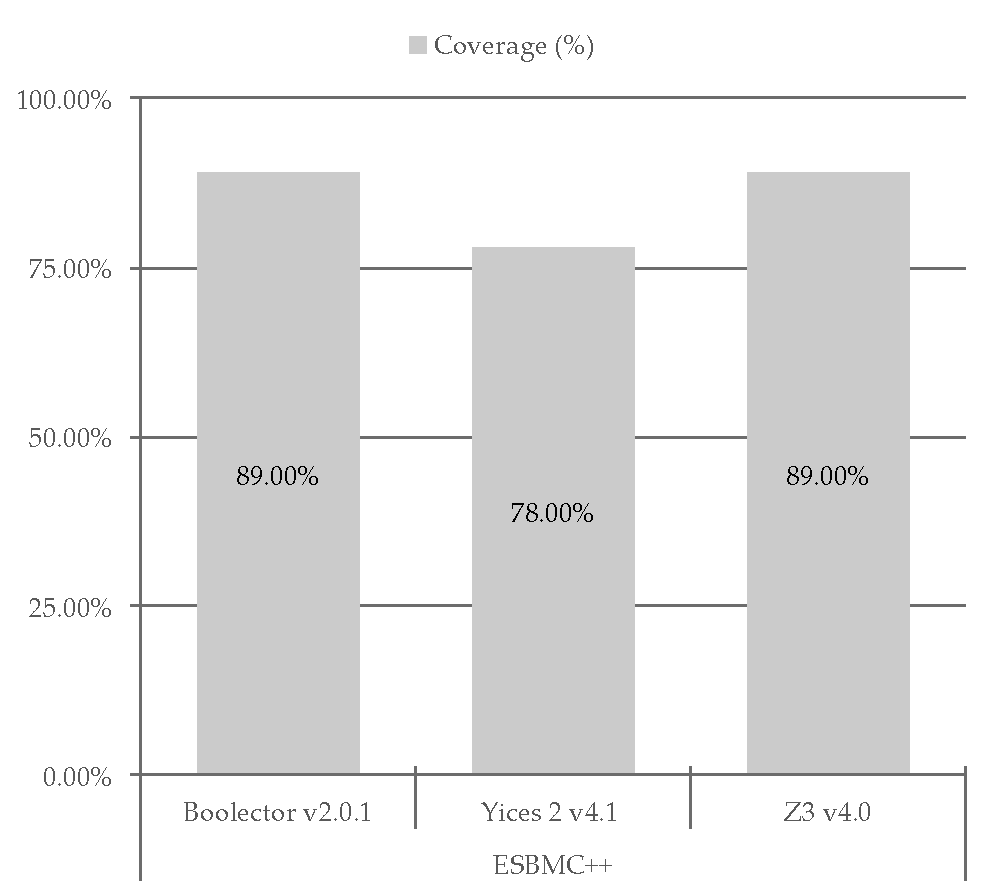
\includegraphics[width=0.45\textwidth]{figuras/qt-coverage.pdf}
\label{subfig-1:coverage}
}
\quad %espaco separador
\subfloat[Tempo de verifica��o]{
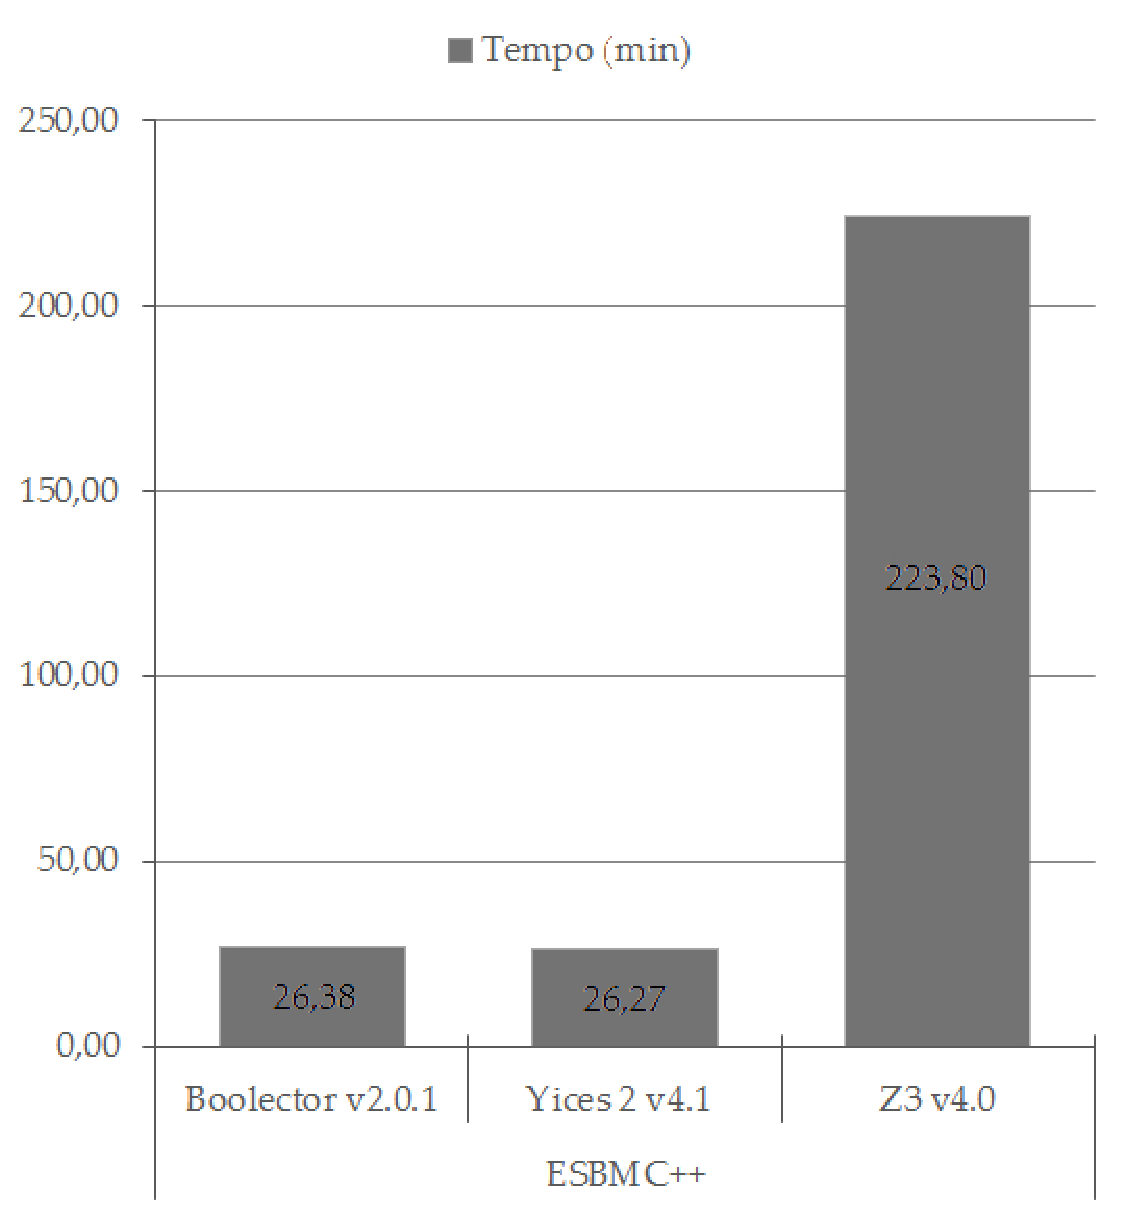
\includegraphics[width=0.45\textwidth]{figuras/qt-time.pdf}
\label{subfig-2:time}
}
\caption{Compara��o entre solucionadores SMT.}
\label{figure:solver-comparison}
\end{figure}

%%%%%%%%%%%%%%%%%%%%%%%%%%%%%%%%%%%%%%%%%%%%%%
\section{Verifica��o dos resultados para o \textit{esbmc--qt}}
\label{sec:evaluation}
%%%%%%%%%%%%%%%%%%%%%%%%%%%%%%%%%%%%%%%%%%%%%%

Todos os casos de teste presentes na su�te de teste \textit{esbmc--qt} foram verificados de forma autom�tica por ESBMC$++$ com o objetivo de analisar a sua corretude e a efic�cia do modelo operacional proposto. Al�m da compara��o entre solucionadores SMT descrita na Se��o~\ref{sec:benchmark}, uma an�lise a cerca do desempenho entre ferramentas de verifica��o distintas tamb�m foi realizada. Como j� mencionado, n�o existe uma ferramenta de verifica��o que verifique o \textit{framework} multiplataforma Qt e nem um modelo operacional semelhante ao proposto neste trabalho (QtOM) utilizando a linguagem C$++$. No entanto, devido � versatilidade do QtOM, tamb�m � poss�vel conect�-lo ao processo de verifica��o de outros verificadores de modelo como LLBMC~\cite{Florian12} e DIVINE~\cite{BBH13}, cuja base deste processo � a tradu��o do c�digo fonte em um representa��o intermedi�ria denominada LLVM. Dessa forma, QtOM � usado como apoio em seus processos de tradu��o, pois o \textit{bitcode} que logo em seguida � produzido, cont�m informa��es a cerca do c�digo fonte utilizado na verifica��o e do modelo operacional proposto (QtOM). Por fim, foi feito uma compara��o em rela��o ao desempenho do LLBMC e ESBMC$++$, que s�o verificadores baseados em t�cnicas SMT, e DIVINE que emprega uma verifica��o de modelos atrav�s de estados expl�citos. Inicialmente, houve uma tentativa de se realizar tamb�m uma compara��o utilizando o verificador CBMC~\cite{CBMC14}, junto com o modelo operacional proposto (QtOM), mas devido � falhas do verificador em rela��o � verifica��o da linguagem C$++$, n�o foi poss�vel realizar as verifica��es previstas, isto j� havia sido relatado em trabalhos anteriores por Ramalho \textit{et al.}~\cite{ECBS13} e Merz \textit{et al.}~\cite{Florian12}, o que ocasionou em sua remo��o durante o processo de avalia��o.

As ferramentas utilizadas foram executadas seguindo tr�s roteiros. Um para ESBMC$++$ que identifica a partir de um arquivo seus par�metros iniciais e realiza sua execu��o, \footnote{esbmc *.cpp -\/-unwind $<$bound$>$  -\/-no-unwinding-assertions -I /home/libraries/ {\tt - \tt -}memlimit 14000000 {\tt - \tt -}timeout 600} outro para LLBMC que usando CLang\footnote{/usr/bin/clang++ -c -g -emit-llvm *.cpp -fno-exceptions}~\cite{CLANG} compila o c�digo fonte desejado criando seu \textit{bitcode} e logo em seguida, tamb�m a partir de um arquivo identifica seus par�metros iniciais e realiza a sua execu��o\footnote{llbmc *.cpp --ignore-missing-function-bodies --max-loop-iterations=$<$bound$>$ --no-max-loop-iterations-checks} e outro para DIVINE que tamb�m pr�-compila os c�digos fontes em C$++$ criando seus respectivos \textit{bitcode}\footnote{divine compile --llvm -o main.bc *.cpp} para que em seguida realize sua verifica��o sobre eles. \footnote{divine verify main.bc --max-time=600 --max-memory=14000 -d} O desdobramento de la�os � definido para cada ferramenta, isto �, o valor de $<$\textit{bound}$>$ varia entre os casos de teste. Por enquanto, o LLBMC n�o suporta tratamento de exce��o e os \textit{bitcodes} que foram criados estavam com a op��o \textit{-fno-exceptions} ativa em seu compilador. Vale ressaltar, que se est� op��o estiver ativa, o LLBMC sempre abortar� durante seu processo de verifica��o.

A Tabela~\ref{table:results-of-ESBMC} mostra os resultados experimentais para as jun��es entre QtOM e LLBMC, DIVINE e ESBMC$++$ usando Boolector como seu principal solucinador SMT. \textit{TC} representa o n�mero de programas Qt/C$++$, \textit{L} representa a quantidade total de linhas de c�digo, \textit{Time} representa o tempo total da verifica��o, \textit{P} representa o n�mero de casos de teste sem defeitos (\textit{i.e.}, resultados positivos corretos), \textit{N} representa o n�mero de casos de teste com defeitos (\textit{i.e.}, resultados negativos corretos), \textit{FP} representa o n�mero falsos positivos obtidos (\textit{i.e.}, a ferramenta relata programas que est�o corretos como incorretos), \textit{FN} representa o n�mero de falsos negativos obtidos (\textit{i.e.}, a ferramenta relata programas incorretos como corretos) e \textit{Fail} representa o n�mero de erros internos obtidos durante a verifica��o (\textit{e.g.}, erros de an�lise). Vale ressaltar que o ESBMC$++$ utilizando Boolector n�o apresenta estouro de mem�ria e tempo em qualquer caso de teste utilizado.

\begin{table}[!htb]
%\begin{adjustwidth}{-0.5cm}{}
\renewcommand\arraystretch{0.95}
\setlength{\tabcolsep}{0.7pt}
\begin{center} {\small
\begin{tabular}{|l|l|r||r|r|r|r|r|r||r|r|r|r|r|r||r|r|r|r|r|r|r|}
\hline
& & & \multicolumn{6}{c||}{ESBMC$++$ v1.25.4}  & \multicolumn{6}{c||}{LLBMC v2013.1}  & \multicolumn{6}{c|}{DIVINE v3.3.2} \\\cline{4-21}
 \textbf{Su�te de teste}    &\textbf{TC}	& \textbf{L}	& \textbf{Time} 	& \textbf{P}  	& \textbf{N}  	& \textbf{FP} 	& \textbf{FN}  & \textbf{Fail}  	& \textbf{Time} 	& \textbf{P}  	& \textbf{N}  	& \textbf{FP} 	& \textbf{FN}  & \textbf{Fail} & \textbf{Time} 	& \textbf{P}  	& \textbf{N}  	& \textbf{FP} 	& \textbf{FN}  & \textbf{Fail} \\\hline
QHash 	   	& 74  	& 1170  	& 117.2   		& 33  	& 33  	& 4  		& 4	  	& 0   			& 37.13   		& 31  	& 37  	& 0  		& 6	  	& 0   		& 1432.5   	& 32  	& 33  	& 0  		& 1	  	& 8 \\ % OK
\hline
QLinkedList 	& 87 		& 1700  	& 77.0  		& 40   	& 39 		& 2   		& 2    	& 4  			& 23.3   		& 18  	& 41 		& 2	  	& 26	  	& 0  	         & 1907.6	   	& 30  	& 42  	& 1  		& 14	  	& 0    \\ % OK
\hline	
QList 		& 124  	& 2317  	& 102.1  		& 53 		& 55 		& 7   		& 9  	 	& 0  			& 19.4   		& 28  	& 56  	& 0	  	& 28	  	& 12  	& 2599.7   	& 52  	& 56  	& 0 		& 4	  	& 12    \\ % OK
\hline
QMap 		& 99  	& 1989  	& 277.2  		& 42 		& 39 		& 10   	& 8   		& 0  			& 406.4   		& 41  	& 46  	& 2  		& 8	  	& 2   		& 2109.9   	& 40  	& 44  	& 0  		& 5	  	& 10   \\ % OK
\hline 
QMultiHash 	& 24  	& 363   	& 186.4   		& 12    	& 12   	& 0   		& 0    	& 0  			& 30.8   		& 12  	& 12  	& 0  		& 0	  	& 0   		& 466.3     	& 13  	& 12  	& 0  		& 0	  	& 0   \\ % OK
\hline
QMultiMap 	& 26   	& 504   	& 136.9		& 13  	& 13   	& 0   		& 0    	& 0  			& 32.0   		& 13  	& 13  	& 0  		& 0	  	& 0   		& 549.9     	& 14  	& 13  	& 0  		& 0	  	& 0    \\ % OK
\hline
QQueue  		& 16   	& 299  	& 191  		& 8   		& 8  		& 0   		& 0    	& 0  			& 3.9   		& 8    	& 8    	& 0  		& 0	  	& 0   		& 339.7     	& 8  	        & 8    	& 0  		& 0	  	& 0    \\ % OK
\hline
QSet 		& 94   	& 1702  	& 500.5  		& 43   	& 43  	& 4  		& 4    	& 0  			& 132.6   		& 40  	& 44  	& 1  		& 5	  	& 4   		& 1897.2   	& 40  	& 41  	& 0  		& 0	  	& 13   \\ % OK
\hline
QStack 		& 12  	& 280  	& 14.5 		& 5 		& 5 		& 0  		& 0   		& 2  			& 2.2   		& 6	   	& 5    	& 1  		& 0	  	& 0   		& 262.1     	&6  	        & 6  	        	& 0  		& 0	  	& 0     \\ % OK
\hline
QVector 		& 152  	& 2582  	&157.3 		& 67  	&68  		& 7  		&8  		& 2  			& 1825.7  		& 44  	& 73  	& 0 		& 29	  	& 6    	& 3057.5   	& 68  	& 72  	& 0  		& 6	  	& 6  \\ % OK
\hline\hline
\textbf{Total} 		& 708 	& 12903 	& 1760		& 316 	& 315	& 34 		& 35   	& 8  			& 2513.5  		& 241  	& 335  	& 6 		& 102	& 24  	& 14722.4   	& 303  	& 327  	& 1  		& 30	  	& 49  \\ % OK
\hline
\end{tabular} }
\end{center}
\caption{Resultados obtidos da compara��o entre ESBMC$++$ v1.25.4 (usando Boolector como solucionador SMT), LLBMC v2013.1 e DIVINE v3.3.2.}
\label{table:results-of-ESBMC}
%\end{adjustwidth}
\end{table}

De acordo com a Tabela~\ref{table:results-of-ESBMC}, apenas $1,1$\% dos casos de teste com o ESBMC$++$ alegaram falhas durante sua verifica��o, isto ocorre quando a ferramenta n�o � capaz de realizar a verifica��o de um determinado programa devido � erros internos encontrados. DIVINE e LLBMC apresentam taxas de falha de $6,9$\% e $3,4$\%, respectivamente, por conta de tais ferramentas n�o conseguirem criar os \textit{bitcodes} dos programas utilizados ou durante a verifica��o realizada foi relatado que houve um estouro de mem�ria ou de tempo. Em rela��o aos resultados $FP$, DIVINE obteve o melhor desempenho seguido por LLBMC e ESBMC$++$. Contudo, ESBMC$++$ obteve a taxa mais baixa em rela��o aos resultados de falsos negativos ($FN$) seguido por DIVINE e por fim LLBMC, isso ocorre devido � forma que os \textit{iterators} est�o implementados no modelo operacional proposto (QtOM), por meio de ponteiros e vetores com o objetivo de simular seus comportamentos de forma real e de acordo com o visto no Cap�tulo~\ref{chapter:container-model}. No entanto, a estrutura criada n�o cobre todos os comportamentos descritos na documenta��o do \textit{framework}. Em particular, quando uma remo��o de um elemento � realizada em um \textit{container} em que existe mais de um \textit{iterator} apontando para ele, todos os \textit{iterators} que apontam para o elemento que foi removido ser�o perdidos. Desta forma, este comportamento afetar� as p�s-condi��es de um programa que influenciam diretamente nos resultados obtidos em rela��o a \textit{FP} e \textit{FN}. Vale ressaltar que vetores e ponteiros t�m sido extensivamente utilizados, de modo a obter estruturas simples, isto �, sem classes e \textit{structs} em sua representa��o o que diminui a complexidade do processo de verifica��o (ver Se��o~\ref{sec:postconditions}). Por fim, os resultados da combina��o entre ESBMC$++$ e QtOM em um verificador robusto, ainda possui algumas lacunas a serem preenchidas a respeito do suporte a linguagem C$++$ como descrito por Ramalho \textit{et al.}~\cite{ECBS13}.

Vale mencionar que o n�vel de complexidade ao se verificar o c�digo fonte de um programa aumenta de acordo com a quantidade de estruturas que possuir \textcolor{red}{(necess�rio mais elementos para determinar a complexidade de um c�digo)}. No entanto, de acordo como mostrado na Figura~\ref{figure:time}, os conjuntos de teste QMap e QSet apresentam os maiores tempos durante o processo de verifica��o ao se utilizar o ESBMC$++$, apesar de QVector ser o mais extenso conjunto de casos de teste existente. Isso acontece por ser analisado a quantidade de la�os presente no programa e n�o somente o n�mero de linhas de c�digo que ele possui, o que afeta diretamente os tempos de verifica��o. Na realidade, as estruturas internas associadas ao modelo operacional das classes \textit{QMap} e \textit{QSet} cont�m mais la�os do que as demais, desta forma, obt�m-se tempos de verifica��o mais longos. Como tamb�m visto na Figura~\ref{figure:time}, o LLBMC apresenta um maior tempo de verifica��o ao se utilizar o conjunto de teste QVector, na qual, isto ocorre devido a $2$ casos de teste em que houve estouro do tempo estimado para que seja realizada a verifica��o. Al�m disso, o DIVINE � a ferramenta que apresenta o menor desempenho entre as citadas, pois, seu processo de cria��o do \textit{bitcode} � mais custoso do que a realiza��o da verifica��o sobre o mesmo. Dessa forma, os conjuntos de teste com mais programas a serem analisados obtiveram os maiores tempos que no caso s�o QVector, QList, QMap, QLinkedList e QSet.

\begin{figure}[htb]
  \centering
  \includegraphics[width=5.5in]{figuras/Time.pdf}
  \caption{Compara��o entre os tempos de verifica��o em rela��o a ESBMC$++$, LLBMC e DIVINE.}
  \label{figure:time}
\end{figure}

A Figura~\ref{figure:coverage} mostra que todos os verificadores obtiveram uma taxa de corbetura acima de 80\% para os \textit{containers} do tipo associativo. Contudo, o LLBMC n�o se manteve com a mesma taxa ao analisar os \textit{containers} do tipo sequencial. Vale ressaltar que todos os casos de teste a partir dos conjuntos de teste QMultiMap e QMultiHash foram verificados corretamente por todos os verificadores utilizados. Os conjuntos de teste QHash, QMap e QSet, por sua vez, apresentaram uma taxa m�dia de $6,7$\% para resultados falsos positivos e falsos negativos, ou seja, de $3$ a $18$ casos de teste dos $267$ casos de teste s�o considerados falsos positivos ou falsos negativos, isso ocorre devido �s limita��es na representa��o interna dos \textit{iterators}. Al�m disso, o LLBMC e DIVINE, respectivamente, n�o conseguiram verificar cerca de $4,5$\% e $13,9$\% dos casos de teste dos \textit{containers} associativos, ou seja, $12$ e $13$ dos $267$ casos de teste n�o conseguiram ser verificados devido �s falhas no processo de cria��o do \textit{bitcode}. Em rela��o aos \textit{containers} do tipo sequencial, LLBMC apresentou baixas taxas de cobertura para os conjuntos de teste QVector, QLinkedList e QList, taxas a cerca de $67,7$\% a $77$\%, ou seja, $84$/$117$ dos $124$/$152$ casos de teste, respectivamente. Al�m disso, cerca de $22,9$\% dos casos de teste ($83$ dos $363$ analisados) apresentaram resultados falsos negativos devido tamb�m � problemas com a representa��o interna dos \textit{iterators}. Vale ressaltar, que cerca de $5$\% dos casos de teste ($18$ dos $363$ analisados) n�o haviam sido verificados por LLBMC, uma vez que n�o foi capaz de criar os \textit{bitcodes} desejados. O ESBMC$++$ e DIVINE, por sua vez, apresentaram uma taxa de erro de no m�ximo de $6,6$\%, ou seja, $24$ dos $363$ casos de teste para os conjuntos de teste QVector, QLinkedList e QList apresentam erros de an�lise em suas p�s-condi��es. Al�m disso, todos os casos de teste dos conjuntos de teste QQueue e QStack foram verificados corretamente, com exce��o de dois casos presentes em QStack, pois, ao se utilizar o Boolector com a ferramenta ESBMC$++$, n�o foi poss�vel obter uma solu��o para as f�rmulas SMT criadas para os casos analisados. 

\begin{figure}[htb]
  \centering
  \includegraphics[width=5.5in]{figuras/Coverage.pdf}
  \caption{Compara��o entre a taxa de cobertura em rela��o a ESBMC++, LLBMC e DIVINE.}
  \label{figure:coverage}
\end{figure}

Os conjuntos de teste QList, QMap, QVector e QSet possuem mais resultados falsos positivos e negativos em seus testes ao se utilizar o ESBMC$++$ do que as outras ferramentas. A taxa de cobertura a cerca dos casos de teste verificados corretamente se encontra em torno de $80$\% a $90$\%, respectivamente, o que demonstra a efic�cia em rela��o a verifica��o realizada uma vez que cada caso de teste verifica caracter�sticas diferentes dos \textit{containers} sequenciais e associativos.

Vale ressaltar que o ESBMC$++$ foi capaz de identificar cerca de $89,3$\% dos erros nos casos de teste utilizados (\textit{i.e.}, $631$ dos $708$ casos de testes utilizados possuem erros), o que demonstra tamb�m a efic�cia da metodologia proposta. Similarmente, LLBMC e DIVINE apresentam, respectivamente, taxas com $81,4$\% e $89$\% (\textit{i.e.}, $576$ e $630$ dos $708$ casos de teste utilizados possuem erros), o que tamb�m demonstra uma boa adequa��o do modelo operacional proposto (QtOM) combinado com outras ferramentas de verifica��o. Como consequ�ncia, a metodologia proposta n�o apenas se limita a uma determinada ferramenta, podendo-se adaptar para aplica��es espec�ficas em que algumas abordagens sejam mais adequedas do que outras. 

%%%%%%%%%%%%%%%%%%%%%%%%%%%%%%%%%%%%%%%%%%%%%%
\section{Verifica��o dos resultados para aplica��es reais}
\label{sec:realqt}
%%%%%%%%%%%%%%%%%%%%%%%%%%%%%%%%%%%%%%%%%%%%%%

Dado que o conjunto de casos de teste proposto possui como objetivo verificar propriedades espec�ficas dos m�dulos pertencentes ao \textit{framework} multiplataforma Qt, tamb�m � necess�rio incluir resultados de verifica��es que envolvam aplica��es reais. Os par�grafos seguintes descrevem as respectivas aplica��es e seus resultados associados.

A aplica��o chamada \textit{Locomaps}~\cite{locomaps} � um exemplo de programa que utiliza o \textit{framework} multiplataforma Qt e exibe imagens de sat�lite, terrenos, mapas de ruas, servi�o de planejamento de mapas em mosaicos e possui um integra��o com GPS \textit{Qt Geo}. Utilizando o mesmo c�digo fonte esta aplica��o pode ser compilada e executada nos principais sistemas operacionais existentes (Mac OS X, Linux e Windows). Est� aplica��o possui duas classes com $115$ linhas de c�digo no total, utilizando Qt/C$++$ e usando cinco APIs diferentes do framework Qt (\textit{QApplication}, \textit{QCoreApplication}, \textit{QDesktopWidget}, \textit{QtDeclarative} e \textit{QMainWindow}). Vale mencionar que o c�digo escrito em Qt/C$++$ desta aplica��o, as APIs e as bibliotecas utilizadas s�o considerados no processo de verifica��o, assim como, as propriedades relacionadas a eles. 

ArcGIS~\cite{ArcGIS} para as for�as armadas � uma plataforma geogr�fica que � utilizado para criar, organizar e compartilhar materiais geogr�ficos com usu�rios que utilizam mapas inteligentes \textit{online}. A partir disso, \textit{GeoMessage Simulator}~\cite{geomessage} possui como entrada de dados arquivos XML e cria em diferentes frequ�ncias datagramas utilizando o protocolo de datagramas por usu�rio (\textit{em ingl�s}, User Datagram Protocol - UDP) para aplica��es ArcGIS e componentes do sistema. \textit{GeoMessage Simulator} tamb�m � uma aplica��o multi-plataforma que cont�m $1209$ linhas de c�digos em Qt/C$++$ que utiliza $20$ diferentes APIs do \textit{framework} multiplataforma Qt englobando v�rias caracter�sticas, tais como o sistema de eventos de Qt, \textit{strings}, manipula��o de arquivos e \textit{widgets}. Vale ressaltar que \textit{GeoMessage Simulator} usa duas classes, \textit{QMutex} e \textit{QMutexLocker}, relacionadas ao m�dulo \textit{Qt Threading} que possui classes para programas concorrentes. Tais classes foram utilizadas na aplica��o para travar ou destravar mutexes e, o mais importante, ESBMC$++$ � capaz de verificar adequadamente esses tipos de estruturas. No entanto, o modelo operacional proposto (QtOM) ainda n�o fornece um suporte completo para o m�dulo \textit{Qt Threading}.

O ESBMC$++$ junto ao modelo operacional proposto (QtOM) foi aplicado para verificar as aplica��es \textit{Locomaps} e \textit{GeoMessage Simulator} buscando verificar as seguintes propriedades: viola��o dos limites de um array, estouros aritm�ticos, divis�o por zero, seguran�a de ponteiro e outras propriedades espec�ficas do \textit{framework} definidas em QtOM de acordo com o Cap�tulo~\ref{chapter:smt-bmc}. Al�m disso, o ESBMC$++$ foi capaz de identificar completamente o c�digo-fonte de cada aplica��o, utilizando cinco diferentes m�dulos de QtOM para \textit{Locomaps} e vinte m�dulos para \textit{GeoMessage Simulator}, ou seja, cada m�dulo de QtOM usado correspondia a uma API utilizada pela aplica��o que seria verificada. O processo de verifica��o de ambas as aplica��es foi totalmente autom�tico e a metodologia proposta levou aproximadamente $6,7$ segundos para gerar $32$ VCs para \textit{Locomaps} e $16$ segundos para gerar $6421$ VCs para \textit{GeoMessage Simulator} em um comum \textit{desktop}. Al�m disso, o ESBMC$++$ n�o relata caso haja qualquer falso negativo, mas foi capaz de encontrar bugs semelhantes em ambas as aplica��es, as quais foram confirmadas pelos desenvolvedores e s�o explicadas abaixo.

\begin{figure}[h]
\centering
\begin{minipage}{0.60\textwidth}
\begin{lstlisting}
int main(int argc, char *argv[]) {
  QApplication app(argc, argv);
  return app.exec();
}
\end{lstlisting}
\end{minipage}
\caption{Fragmento de c�digo do arquivo principal da aplica��o \textit{Locomaps}.}
\label{fig:Fig6}
\end{figure}

A Figura~\ref{fig:Fig6} mostra um fragmento de c�digo retirado do principal arquivo da aplica��o \textit{Locomaps} que utiliza a classe \textit{QApplication} que est� presente no m�dulo \textit{QtWidgets}. Nesse caso em particular, se o par�metro $argv$ n�o for corretamente inicializado, logo o construtor ao ser chamado pelo objeto $app$ n�o � executado de forma correta acarretando em falhas na aplica��o (veja a linha $2$, na Figura~\ref{fig:Fig6}). A fim de verificar esta propriedade, o ESBMC$++$ analisa 2 assertivas em rela��o aos par�metros de entrada da aplica��o (veja as linhas $4$ e $5$, na Figura~\ref{fig:Fig7}), avaliando-as como pr�-condi��es. Um erro semelhante tamb�m foi encontrado na aplica��o \textit{GeoMessage Simulator} e uma maneira poss�vel para corrigir tal erro � sempre verificar, com instru��es condicionais, se $argv$ e $argc$ s�o argumentos v�lidos antes de utiliza-las em uma opera��o.\\\\\\

\begin{figure}[h]
\centering
\begin{minipage}{0.60\textwidth}
\begin{lstlisting}
class QApplication {
  ...
  QApplication( int & argc, char ** argv ){
  __ESBMC_assert(argc > 0, ``Invalid parameter'');
  __ESBMC_assert(argv != NULL, ``Invalid pointer'');
  this->str = argv;
  this->_size = strlen(*argv);
  ...
 }
 ...
};
\end{lstlisting}
\end{minipage}
\caption{Modelo operacional para o construstor de $QApplication$().}
\label{fig:Fig7}
\end{figure}

%%%%%%%%%%%%%%%%%%%%%%%%%%%%%%%%%%%%%%%%%%%%%%
\section{Verifica��o da conformidade de QtOM}
\label{sec:conformance}
%%%%%%%%%%%%%%%%%%%%%%%%%%%%%%%%%%%%%%%%%%%%%%
Todos os processos, fun��es, APis, ferramentas e especifica��es necess�rias para o desenvolvimento de aplica��es que utilizam o \textit{framework} multiplataforma Qt s�o descritas por \textit{The Qt Developers} em~\cite{qtdevelopers}. Na verifica��o de modelos, as aplica��es analisadas se utilizam de fun��es disponibilizadas pelo ambiente de verifica��o criado com o objetivo de garantir a exatid�o da verifica��o, ou seja, se obter uma an�lise de forma correta. Para que isso ocorra, o comportamento do sistema desenvolvido (modelo operacional) deve ser o mesmo do sistema real (framework) analisado. 

Inicialmente, foi realizado uma an�lise sobre todos os casos de testes utilizados em \textit{esbmc--qt} com intuito de verificar a imparcialidade e a confiabilidade das aplica��es utilizadas. Todos os casos de teste analisados foram desenvolvidos utilizando a linguaguem C++ junto com as fun��es disponibilizadas pelo \textit{framework} Qt, onde cada implementa��o usa as estruturas de dados e fun��es presente em Qt \textit{containers} em todas as condi��es poss�veis de acordo com \textit{The Qt Documentation}~\cite{qtdocumentation}. Cada caso de teste proporciona uma falha e um sucesso de acordo com a estrutura ou fun��o empregada. Logo em seguida, todos os casos de testes presentes em \textit{esbmc--qt} foram compilados e executados utilizando o ambiente de desenvolvimento do Qt denominado QtCreator. QtCreator � um ambiente de desenvolvimento integrado (IDE) multiplataforma utilizado por desenvolvedores para criar diversas aplica��es que utilizam o \textit{framework} Qt para desktops, sistemas embarcados e plataformas de dispositivos m�veis. � um ambiente de desenvolvimento dispon�vel para Linux, OS X e Windows~\cite{qtcreator}. Dessa forma, se obteve um comportamento base de Qt \textit{containers} que seria comparado ao comportamento do modelo operacional proposto (QtOM) com o objetivo de verificar o n�vel de semelhan�a entre ambos, visto que n�o h� outra ferramenta ou modelo operacional desenvolvido at� o momento. Por fim, os mesmo casos de teste compilados e executados por QtCreator foram compilados e executados por Clang com o modelo operacional proposto (QtOM) intregado a ele com o intuito de se determinar o seu comportamento.

A Figura~\ref{fig:conformance} mostra o resultado da compara��o descrita anteriormente, assim como, em testes anteriores os conjuntos de testes est�o divididos em \textit{containers} associativos compostos por QHash, QSet, QMap, QMultiHash e QMultiMap e \textit{containers} sequenciais compostos por QList, QQueue, QLinkedList, QStack e QVector. Vale ressaltar que QtCreator por ser o ambiente de desenvolvimento padr�o para cria��o de aplica��es que usam o \textit{framework} Qt, obteve um n�vel de conformidade de 100\% em todos os conjuntos de testes que comp�e \textit{esbmc--qt} em todas as condi��es poss�veis de acordo com \textit{The Qt Documentation}~\cite{qtdocumentation}. Entretanto, ao se analisar o comportamento do compilador Clang junto com o modelo operacional proposto (QtOM), se obtem um n�vel de conformidade com m�dia de 94,320\% em todos os conjuntos de testes que comp�e \textit{esbmc--qt} em todas as condi��es poss�veis de acordo com \textit{The Qt Documentation}~\cite{qtdocumentation}. 

Ao se analisar de modo particular, os conjuntos de testes QMultiHash, QMultiMap, QQueue, QStack obtiveram um n�vel de 100\% de semalhan�a comparado aos resultados obtidos por QtCreator. O conjunto de teste QList obteve o menor n�vel de semelhan�a em rela��o a QtCreator com 84,677\%, isso ocorreu devido algumas fun��es presente na classe \textit{QList} n�o possuirem uma representa��o dentro do modelo operacional proposto, o mesmo ocorreu com o conjunto de teste QVector que obteve um n�vel de semelhan�a de 90,789\% e considero o conjunto de teste com o maior n�mero de casos de teste. Vale ressaltar que o modelo operacional desenvolvido � usado junto com ferramentas de verifica��o que possuem suas limita��es em rela��o as linguagens bases utilizadas o que consequentemente afeta na cria��o das representa��es de algumas fun��es, n�o sendo poss�vel a cria��o de certas representa��es (\textit{i.e.} fromSet, fromStdList, fromVector, etc).


\begin{figure}[htb]
  \centering
  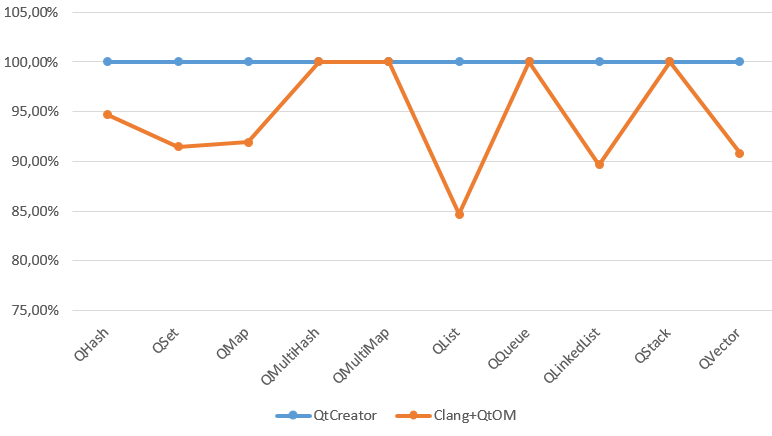
\includegraphics[width=5.5in]{figuras/conformance.png}
  \caption{Compara��o entre o comportamento de QtCreator e Clang+QtOM parar medir a conformidade de QtOM.}
  \label{fig:conformance}
\end{figure}



%%%%%%%%%%%%%%%%%%%%%%%%%%%%%%%%%%%%%%%%%%%%%%
\section{Resumo}
%%%%%%%%%%%%%%%%%%%%%%%%%%%%%%%%%%%%%%%%%%%%%%

De acordo com o embasamento te�rico realizado pelos cap�tulos anteriores em rela��o as t�cnicas SMT utilizadas, o processo de verifica��o de ESBMC++ e o modelo operacional para \textit{Qt Container} desenvolvido. Neste cap�tulo, inicialmente foi descrito como foi constru�da a configura��o dos experimentos realizados, com o intuito de avaliar a efic�cia da metodologia proposta a cerca da verifica��o de programas que utilizam o \textit{framework} multiplaforma Qt, a partir de uma su�te de testes denomidado \textit{esbmc--qt} que cont�m todos os casos de teste utilizadas na atual avalia��o. O \textit{esbmc--qt} cont�m $711$ programas Qt/C$++$ que de acordo com os experimentos realizados � poss�vel garantir que $353$ dos $711$ casos de teste cont�m erro (\textit{i.e.}, $49.65$\% do casos de teste analisados cont�m erro) e $358$ casos de teste n�o possuem falhas (\textit{i.e.}, $50.35$\% dos casos de teste analisados s�o considerados corretos). 

Em seguida, foi descrito como foi realizado e avaliado a compara��o entre os solucionadores SMT utilizados (Z3, Boolector e Yices 2) junto com o ESBMC$++$ utilizando programas Qt/C$++$ sequenciais. Isso foi realizado, pois, solucionadores SMT podem afetar fortemente os resultados obtidos, uma vez que n�o existe homogeneidade em rela��o a abordagem de implementa��o e respectivas heur�sticas. Sendo assim, Yices 2 obteve os piores resultados, apresentando uma taxa de cobertura de $78$\% e um tempo de verifica��o de $26,27$ minutos mas tanto Z3 quanto Boolector apresentaram uma taxa de cobertura de $89$\% com tempos de verifica��o de $223,6$ minutos e $26,38$ minutos, respectivamente. Por fim, Boolector mostrou-se $8,5$ vezes mais r�pido do que o solucionador Z3, apesar da mesma precis�o de ambos. 

Tamb�m foram descrito os resultados obtidos a cerca da verifica��o de todos os casos de teste presentes na su�te de teste \textit{esbmc--qt} utilizando ferramentas de verifica��o distintas (ESBMC$++$, LLBMC e DIVINE) com o objetivo de analisar a corretude e a efic�cia do modelo operacional proposto junto dessas ferramentas. Cada processo de verifica��o e as limita��es das ferramentas s�o descritos. Vale ressaltar que o ESBMC$++$ foi capaz de identificar cerca de $89,3$\% dos erros nos casos de teste utilizados (\textit{i.e.}, $631$ dos $708$ casos de testes utilizados possuem erros), LLBMC e DIVINE apresentam, respectivamente, taxas com $81,4$\% e $89$\% (\textit{i.e.}, $576$ e $630$ dos $708$ casos de teste utilizados possuem erros). Como consequ�ncia, a metodologia proposta n�o apenas se limita a uma determinada ferramenta, podendo-se adaptar para aplica��es espec�ficas em que algumas abordagens sejam mais adequedas do que outras. 

Por fim, foi descrito os resultados obtidos atr�ves da verifica��o de 2 aplica��es reais \textit{Locomaps} e \textit{GeoMessage Simulator} utilizando QtOM. O ESBMC$++$ junto ao modelo operacional proposto (QtOM) foi aplicado para verificar as aplica��es \textit{Locomaps} e \textit{GeoMessage Simulator} buscando verificar as seguintes propriedades: viola��o dos limites de um array, estouros aritm�ticos, divis�o por zero, seguran�a de ponteiro e outras propriedades espec�ficas do \textit{framework} definidas em QtOM. O processo de verifica��o de ambas as aplica��es com a metodologia proposta levou aproximadamente $6,7$ segundos para gerar $32$ VCs para \textit{Locomaps} e $16$ segundos para gerar $6421$ VCs para \textit{GeoMessage Simulator} em um comum \textit{desktop} onde ambas aplica��es possuiam o mesmo erro.

%Outros topicos
%%%%%%%%%%%%%%%%%%%%%%%%%%%%%%%%%%%%%%%%%%%%%%%
\section{Algoritmo \textit{K-Induction}}
\label{sec:k-induction-algorithm}
%%%%%%%%%%%%%%%%%%%%%%%%%%%%%%%%%%%%%%%%%%%%%%

Algoritmo

%%%%%%%%%%%%%%%%%%%%%%%%%%%%%%%%%%%%%%%%%%%%%%
\chapter{Conclus�es}
\label{chapter:conclusion}
%%%%%%%%%%%%%%%%%%%%%%%%%%%%%%%%%%%%%%%%%%%%%%

A abordagem proposta neste trabalho tem como objetivo verificar programas que utilizam o \textit{framework} multiplataforma Qt desenvolvido em Qt/C$++$, usando um modelo operacional denominado de QtOM que se utiliza de pr� e p�s-condi��es, simula��o de caracter�sticas (por exemplo, como os elementos que possuem valores s�o manipulados e armazenados) e tamb�m da forma como s�o utilizados em dispositivos de eletr�nica de consumo. A forma como o modelo operacional proposto foi implementado, foi tamb�m descrita, levando-se em considera��o que � usado para verificar \textit{containers} de tipos sequenciais e associativos. Al�m disso, uma aplica��o \textit{touchscreen} baseada em Qt que utiliza mapas de navega��o, imagens de sat�lite e dados de terrenos~\cite{locomaps} e outra que gera \textit{datagramas broadcast} UDP com base em arquivos XML~\cite{geomessage} foram verificadas usando o ESBMC$++$ com o QtOM. Desta forma, foi mostrado o potencial da abordagem proposta para a verifica��o de aplica��es reais baseadas no \textit{framework} Qt. 

Este trabalho possui como contribui��o principal a constru��o de um modelo operacional denominado QtOM que oferece suporte � \textit{containers} sequenciais e associativos que utilizam o \textit{framework} multiplataforma Qt. Os experimentos que foram realizados envolvem programas em Qt/C$++$ com caracter�sticas oferecidas pelas classes \textit{container} do \textit{framework} multiplataforma Qt e abordam todas as condi��es poss�veis de acordo com \textit{The Qt Documentation}~\cite{qtdocumentation}.

%%%%%%%%%%%%%%%%%%%%%%%%%%%%%%%%%%%%%%%%%%%%%% Na verdade, os resultados das  verifica��es realizadas demonstram a efici�ncia e a efic�cia da abordagem BMC baseada em SMT proposta com ESBMC$++$ a cerca da verifica��o de programas que utilizam o framework Qt tamb�m � apresentado um conjunto de teste com uma taxa de sucesso de $89,3$\% com um tempo de $1760$ segundos de verifica��o.

Al�m disso, tamb�m foram avaliados o desempenho dos solucionadores Z3, Boolector e Yices 2, dado que eles foram utilizados no processo de verifica��o dos programas que utilizam o \textit{framework} multiplataforma Qt com ESBMC$++$ e o modelo operacional proposto (QtOM). Como resultado, o Boolector apresentou a maior taxa de cobertura dos programas verificados com um menor tempo de verifica��o e o ESBMC$++$ apresentou uma taxa de sucesso de $89,3$\% para o conjunto de teste utilizado com um tempo de $1760$ segundos de verifica��o. Ainda foi avaliado o n�vel de conformidade do modelo operacional proposto (QtOM) atr�ves da compara��o de entre o comportamento real do \textit{framework} e o comportamento do modelo operacional desenvolvido. Como resultado, QtOM obteve um n�vel de conformidade com m�dia de 97,827\% e de maneira particular os conjuntos de teste QHash, QSet, QMap, QMultiHash, QMultiMap, QList, QQueue, QLinkedList, QStack, QVector obtiveram n�veis de conformidade de 94,667\%, 97,872\%, 91,919\%, 100,000\%, 100,000\%, 97,580\%, 100,000\%, 98,850\%, 100,000\%, 97,378\%, respectivamente. O conjunto de teste QMap obteve o menor n�vel de conformidade devido a problemas em suas representa��es e QLinkedList foi o conjunto de teste que obteve o maior n�vel de conformidade entre os conjuntos que n�o obtiveram um n�vel igual a 100\%.  

Por fim, outra fundamental contribui��o � a integra��o de QtOM dentro do processo de verifica��o de outro dois diferentes verificadores de modelo conhecidos como LLBMC e DIVINE, demonstrando a versatilidade do QtOM. Esse tipo de alternativa tamb�m demonstra resultados importantes, uma vez que LLBMC detectou $95$\% dos erros existentes com um tempo de verifica��o de $2513$ segundos e o DIVINE encontrou $92$\% dos erros existentes com um tempo de verifica��o em torno de $1760$ segundos. Contudo, o LLBMC possui a maior taxa de resultados incorretos entre as ferramentas utilizadas com $18,6$\%, seguido de DIVINE com $11,3$\% e por fim ESBMC$++$ com $10,9$\%. Vale ressaltar que o DIVINE � $7$ vezes mais lento do que as demais ferramentas utilizadas, seguido pelo LLBMC e ESBMC$++$, respectivamente. Em resumo, o QtOM pode ser integrado em uma ferramenta de verifica��o adequada e utilizado para verificar programas reais que est�o escritos em C$++$/Qt para cen�rios espec�ficos e aplica��es.

%%%%%%%%%%%%%%%%%%%%%%%%%%%%%%%%%%%%%%%%%%%%%%
\section{Trabalhos Futuros}
%%%%%%%%%%%%%%%%%%%%%%%%%%%%%%%%%%%%%%%%%%%%%%

Como trabalhos futuros, o modelo operacional proposto (QtOM) ser� estendido com o objetivo de oferecer suporte � verifica��o de programas multi-tarefas que utilizam o \textit{framework} multiplataforma Qt. Al�m disso, mais classes e bibliotecas ser�o adicionadas com o intuito de aumentar a cobertura da verifica��o em rela��o ao \textit{framework} multiplataforma Qt e dessa forma validar suas respectivas propriedades. Novas ferramentas para medi��o de desempenho do modelo operacional proposto e novos testes de conformidade ser�o inclu�dos, a fim de verificar se as rotinas espec�ficas est�o de acordo com as limita��es de tempo. Por fim, ser� investigada a verifica��o por indu��o matem�tica no ESBMC$^{QtOM}$ para provar a corretude de programas Qt~\cite{Gadelha2015,RochaICB15}.

\bibliographystyle{abntex2-num}
\bibliography{bibliografia/bibliografias}

%%%%%%%%%%%%%%%%%%%%%%%%%%%%%%%%%%%%%%%%%%%%%%
\appendix
%%%%%%%%%%%%%%%%%%%%%%%%%%%%%%%%%%%%%%%%%%%%%%

\chapter{Publica��es}

\section{Referente � Pesquisa}

\begin{itemize}
 \item \textcolor{red}{AINDA FALTA MODIFICAR ESSA PARTE}
 \item \textbf{Mikhail Ramalho}, Mauro Freitas, Felipe Sousa, Hendrio Marques, Lucas Cordeiro e Bernd Fischer. \textit{SMT-Based Bounded Model Checking
 of C++ Programs}. \textbf{20th IEEE International Conference and Workshops on the Engineering of Computer Based Systems}, Phoenix, 2013. p. 147-156.
 \item \textbf{Mikhail Ramalho}, Lucas Cordeiro, Andr� Cavalcante e Vicente Lucena. \textit{Verifica��o Baseada em Indu��o Matem�tica para
 Programas C/C++}. \textbf{III Simp�sio Brasileiro de Engenharia de Sistemas Computacionais}. Niter�i, Rio de Janeiro.
\end{itemize}

\section{Contribui��es em outras Pesquisas}

\begin{itemize}
 \item \textcolor{red}{AINDA FALTA MODIFICAR ESSA PARTE}
 \item Mauro L. de Freitas, \textbf{Mikhail Y. R. Gadelha}, Lucas C. Cordeiro, Waldir S. S. J�nior e Eddie B. L. Filho. \textit{Verifica��o de
 Propriedades de Filtros Digitais Implementados com Aritm�tica de Ponto Fixo}. \textbf{XXXI Simp�sio Brasileiro de Telecomunica��es - SBrT}, 2013.
\end{itemize} 


\end{document}

